%---------------------------------------------------
% University of Sussex thesis template
% Last Edit by Fabrizio Miano, Oct 2017
%---------------------------------------------------
\RequirePackage[l2tabu,orthodox]{nag} 
\RequirePackage{mathpazo}
\documentclass[a4paper,11pt,oneside]{book}
\usepackage{booktabs}
\usepackage{hepunits}
\usepackage{physics}
\usepackage{latex/atlasphysics}
\usepackage{enumerate}
\usepackage{epigraph}
\usepackage{placeins}
\usepackage[font=footnotesize,hang]{caption} % footnotes
\usepackage{multicol} % multicolumn text
\usepackage{wrapfig} % figures wrapped in text
\usepackage{booktabs} % lines for tables
\usepackage{lineno} % Line Numbers 
\usepackage[utf8]{inputenc}
\usepackage{subfig}
%\usepackage[Sonny]{fncychap} % header style 
%Options: Sonny, Glenn, Conny, Rejne, Bjornstrup
\setcounter{secnumdepth}{4}

%---------------------------------------------------
% LINE SPACING
%---------------------------------------------------
\newcommand{\linespacing}{1.5}
\renewcommand{\baselinestretch}{\linespacing}
\def\mubar{\ensuremath{\langle\mu\rangle}}

%---------------------------------------------------
% BIBLIOGRAPHY STYLE
%---------------------------------------------------
\bibliographystyle{latex/atlasBibStyleWithTitle}

%---------------------------------------------------
%   DOCUMENT VARIABLES
%   Fill in the lines below to enter your information into the thesis template
%   Each of the commands can be cited anywhere in the thesis
%---------------------------------------------------
\newcommand{\myTitle}{Optimisation studies and background estimation in searches for the supersymmetric partner of the top quark in all-hadronic final states with the ATLAS Detector at the LHC}
\newcommand{\mySubtitle}{NO SUBTITLE\xspace}
\newcommand{\myDegree}{Doctor of Philosophy \xspace}
\newcommand{\myName}{Fabrizio \textsc{Miano}\xspace}
\newcommand{\myProf}{Dr. Fabrizio \textsc{Salvatore}\xspace}
\newcommand{\myOtherProf}{Prof. Antonella \textsc{De Santo}\xspace}
\newcommand{\mySupervisor}{Dr. Fabrizio \textsc{Salvatore}\xspace}
\newcommand{\myDepartment}{\href{http://www.sussex.ac.uk/epp/}{Experimental Particle Physics Research Group\xspace}}
\newcommand{\myFaculty}{\href{http://www.sussex.ac.uk/mps/}{School of Mathematical and Physical Sciences\xspace}}
\newcommand{\myUni}{University of Sussex\xspace}
\newcommand{\myLocation}{Brighton\xspace}
\newcommand{\myTime}{June 2018\xspace}
\newcommand{\myVersion}{version 1.0\xspace}

%---------------------------------------------------
% USEFUL COMMANDS
%---------------------------------------------------
\newcommand{\ie}{i.\,e.}
\newcommand{\Ie}{I.\,e.}
\newcommand{\eg}{e.\,g.}
\newcommand{\Eg}{E.\,g.}
\newcommand{\Width}{1.5}
\newcommand{\Height}{2.5}
%\newcommand{\DeltaX}{5}
\newcommand{\NumberOfVerticalLines}{4}
\newcommand*{\Rectangle}[4][]{%
    % #1 = draw/fill options
    % #2 = width
    % #3 = height
    % #4 = number of vertical lines
    \draw [#1] (0,0) rectangle (#2,#3);
    \pgfmathsetmacro{\DeltaX}{#2/#4}%
    \foreach \x in {1,...,#4} {
        \pgfmathsetmacro{\NewX}{\DeltaX*\x}
        \draw ($(0,0)+(\NewX,0)$) -- ($(0,0)+(\NewX,#3)$);
    }
}

%---------------------------------------------------
% OTHER FORMATTING/LAYOUT DECLARATIONS
%---------------------------------------------------
% Graphics
\usepackage{color}
\usepackage{feynmp}
\usepackage[pdftex]{graphicx}
%\renewcommand{\includegraphics}[2][]{\fbox{}}
\DeclareGraphicsRule{*}{mps}{*}{} 
\usepackage{pgfplots}
\pgfplotsset{compat=1.14}
\usepackage{amsmath}
\usepackage{commath}
\usepackage{amssymb}
\usepackage[british]{babel}
\usepackage{multirow}
\usepackage{tikz}
\usepackage{tikz-3dplot}
\usepackage{cancel}
\usetikzlibrary{decorations.markings,calc,shapes,arrows}

%---------------------------------------------------
% MARGINS
%---------------------------------------------------
% The left-hand-side should be 40mm.  The top and bottom margins should be
% 25mm deep.  The right hand margin should be 20mm.
\usepackage[a4paper,top=2.5cm,bottom=2.5cm,left=4cm,right=2cm,headsep=10pt]{geometry}
\flushbottom
\usepackage{fancyhdr}
% Pages should be numbered consecutively thorugh the main text.  Page numbers
% should be located centrally at the top of the page.
\pagestyle{fancy}
    \fancyhf{} 
    \renewcommand{\sectionmark}[1]{\markright{{\textit{\thesection\ #1}}}}
    \lhead{}
    \rhead{\nouppercase{\rightmark}}
    \chead{\thepage}
    \cfoot{}
    \lfoot{}
    \rfoot{}
    \renewcommand{\headrulewidth}{0.4pt}
    \renewcommand{\footrulewidth}{0.4pt}

% Even the first page of the chapter
\fancypagestyle{plain}{% % <-- this is new
    \fancyhf{} 
    %\rhead{\nouppercase{\rightmark}}
    \chead{\thepage}
    %\fancyfoot[LE,RO]{\thepage} % same placement as with page style "fancy"
    \renewcommand{\headrulewidth}{0pt}
    \renewcommand{\footrulewidth}{0pt}
    }

%---------------------------------------------------
% HYPERREF
%---------------------------------------------------
\usepackage[colorlinks,pagebackref,pdfusetitle,
            urlcolor=blue,citecolor=blue,linkcolor=blue,
            bookmarksnumbered,plainpages=false]{hyperref}
% For print version, use this instead:
%\usepackage[pdfusetitle,bookmarksnumbered,plainpages=false]{hyperref}
%\usepackage{backref}
%\renewcommand{\backrefpagesname}{Cited on}
%---------------------------------------------------

\raggedbottom

%Check for unreferenced figures
%\usepackage{refcheck}
\graphicspath{{./figures/}}

%---------------------------------------------------
% BEGIN DOCUMENT
%---------------------------------------------------
\begin{document}
    %---------------------------------------------------
    % Line numbers
    %---------------------------------------------------
    \linenumbers

    %---------------------------------------------------
    % PREAMBLE: roman page numbering i, ii, iii, ...
    %---------------------------------------------------
    \frontmatter
    \pagenumbering{roman}

    %%%%%%%%%%%%%%%%%%%%%%%%%%%%
%% TITLE PAGE: The title page should give the following information:
%%	(i) the full title of the thesis and the sub-title if any;
%%	(ii) the full name of the author;
%%	(iii) the qualification aimed for;
%%	(iv) the name of the University of Sussex;
%%	(v) the month and year of submission.
% \pagestyle{empty}
\begin{titlepage}
	\begin{center}

		\includegraphics[width=4.5cm]{uslogo.eps} \\ \medskip
		\vspace*{.05\textheight}
		\textsc{\Large Doctoral Thesis}\\%[0.5cm] % Thesis type

		\rule{.9\linewidth}{.6pt}\\[0.4cm]
		{\huge \myTitle \par}\vspace{0.4cm} %\bigskip % Thesis title
		\rule{.9\linewidth}{.6pt}\\[1cm] 

		\large \textit{A thesis submitted in fulfillment of the requirements\\ for the degree of Doctor of Philosophy}\\[0.5cm] % University requirement text
		\textit{in the}\\[0.5cm]
		\myDepartment\\ \myFaculty\\[1cm]
	
		\begin{minipage}{.45\linewidth}
			\begin{flushleft} %\large
			\emph{Author:}\\
			\href{https://uk.linkedin.com/in/fabriziomiano}{\myName} % Author name - remove the \href bracket to remove the link
			\end{flushleft}
		\end{minipage}
		\hfill
		\begin{minipage}{.45\linewidth}
			\begin{flushright} %\large
			\emph{Supervisor:} \\
			\href{http://www.sussex.ac.uk/profiles/168614}{\mySupervisor}%\\ % Supervisor name - remove the \href bracket to remove the link  
			\end{flushright}
		\end{minipage}\\ [0.5cm]

		{\large \today}\\%[3cm] % Date
		 
		\vfill
	\end{center}
\end{titlepage}
    \newpage \vspace*{8cm}
\pdfbookmark[0]{Dedication}{Dedication} % Bookmark name visible in a PDF viewer
\thispagestyle{empty}

\begin{flushright}
   \emph{To Mum, Dad, and Eleonora whose support has always been constant.}
\end{flushright}

\begin{flushright}
   \emph{To Martina, whose affection played a major role during the most difficult times of my life.}
\end{flushright}

\begin{flushright}
   \emph{To my friends, lovely bunch of outlandish characters.}
\end{flushright} % Dedication page
    % Acknowledgements 

\thispagestyle{empty}
\pdfbookmark[0]{Acknowledgements}{Acknowledgements} % Bookmark name visible in a PDF viewer
%\epigraph{\emph{Have no fear for atomic energy `cause none of them can stop the time}}{Robert Nesta Marley}

\begin{center}
	\noindent{\Huge\textit{Acknowledgments}}
\end{center}

\vspace*{.05\textheight}

\noindent Thanks to every single thing that went wrong. It made me stronger. 

% Fab, antonella, Iacopo, 
% mentoring Kerim, Mark, Zara, Giuseppe 

% and the other EPP student. Suf, Mark and James, Ed,  

% ben sowden (big support at CERN) 

% family, massimo, lucio (Ps4)  % Acknowledgements page
    % Declaration

\thispagestyle{empty}
\pdfbookmark[0]{Declaration}{declaration} % Bookmark name visible in a PDF viewer

\begin{center}
	\noindent{\Huge\textit{Statement} \par}
\end{center}

\vspace*{.05\textheight}


\noindent I, \myName, hereby declare that this thesis, titled ``\myTitle'', has not been and will not be, submitted in whole or in part to another University for the award of any other degree.

\bigskip
 
\textit{\myLocation, \myTime}

\bigskip

\begin{flushright}
 	\begin{tabular}{l}
	\hline \\ 
	\centering \myName 
 	\end{tabular}
\end{flushright}
 % Declaration
    % % Abstract

\thispagestyle{empty}
\pdfbookmark[0]{Abstract}{Abstract} % Bookmark name visible in a PDF viewer

\begin{center}
%	\bigskip

    {\normalsize \href{http://www.sussex.ac.uk/}{\myUni} \\} % University name in capitals
    {\normalsize \myFaculty \\} % Faculty name
    {\normalsize \myDepartment \\} % Department name
    \bigskip\vspace*{.02\textheight}
    {\Large \textsc{Doctoral Thesis}}\par
    \bigskip
    
    {\rule{\linewidth}{1pt}\\%[0.4cm]
    \Large \myTitle \par} % Thesis title
    \rule{\linewidth}{1pt}\\[0.4cm]
    
    \bigskip
	{\normalsize by \myName \par} % Author name
    \bigskip\vspace*{.06\textheight}
\end{center}

    {\centering\Huge\textsc{\textbf{Abstract}} \par}
    \bigskip



    \noindent This thesis presents the search for the supersymmetric partner of the top quark in $\sqrt{s}=13$ \TeV\ proton-proton collisions at the LHC using data collected by the ATLAS detector in 2015 and 2016. Results were interpreted considering natural supersymmetric extensions of the Standard Model in $R$-parity conserving decays. Events characterised by four or more jets and missing transverse momentum in the final states were selected. The performances of the tracking algorithms used by the ATLAS online trigger were studied. Optimisation studies of the search regions to increase the sensitivity to supersymmetric signals were performed and data-driven techniques to estimate Standard Model backgrounds were employed. The agreement between data and background predictions was extensively checked and the extrapolations from background-enriched regions to signal-enriched regions were validated. The analysis yielded no significant excess therefore exclusion limits on various models were set.


 % Abstract page

    %---------------------------------------------------
    % TABLE OF CONTENTS, LISTS OF TABLES & FIGURES
    %---------------------------------------------------
    \newpage
    \pdfbookmark[0]{Contents}{contents_bookmark}
    \tableofcontents
    \listoftables
    \phantomsection
    %\addcontentsline{toc}{chapter}{List of Tables}
    \listoffigures
    \phantomsection
    %\addcontentsline{toc}{chapter}{List of Figures}

    %---------------------------------------------------
    % MAIN THESIS TEXT: arabic page numbering 1, 2, 3, ...
    %---------------------------------------------------
    \newpage
    \pagenumbering{arabic}

    %---------------------------------------------------
    % THESIS CONTENT - CHAPTERS
    %---------------------------------------------------
    \mainmatter
    \chapter*{Introduction}
\addcontentsline{toc}{chapter}{Introduction}
\markboth{}{Introduction}

Last thing to write

    \chapter{The Standard Model of particle physics and Supersymmetry}
\label{ch:theory} 
\epigraph{\emph{A theory is something nobody believes, except the person who made it. An experiment is something everybody believes, except the person who made it.}} {Albert Einstein}

	In this chapter, an overview of the Standard Model (SM) of particle physics will be presented in Section~\ref{sec:SMov} together with its limitations in Section~\ref{sec:SMlim} and the need of an extension. One of the most popular, supersymmetry, will be discussed in Section~\ref{sec:SUSY} where, an overview of the theory, together with the motivations behind its success, will be presented in Section~\ref{sec:whySUSY}, followed by the description of the Minimal Supersymmetric Standard Model (MSSM) in Section~\ref{sec:MSSM}, and finally, the phenomenology of supersymmetry, with particular attention on third-generation supersymmetry, as it is the most relevant theoretical support to the analyses presented in this work, will be discussed in Section~\ref{sec:SUSYPheno}.



	\section{The Standard Model}
	\label{sec:SMov}

		The SM is an effective theory that aims to provide a general description of fundamental particles and their interactions. Unfortunately, our understanding of nature is still limited due to some opened question the SM is not able to answer to.

		\begin{wrapfigure}{R}{.5\textwidth}
		%\begin{figure}[!htb]
			\centering
				\includegraphics[width=.5\textwidth]{theory/sm}
			\caption{\label{fig:sm_el_part} The elementary particles of the Standard Model. From the outermost to the innermost; fermions (quarks, top-half wheel, leptons, bottom-half wheel), vector bosons, and the Higgs boson.} %Any given point around the bottom of the hat gives the lowest-energy state.}
		\end{wrapfigure}		

		The 20$^{th}$ century can be considered a quantum revolution. Several experiments led to discoveries which were found to be, together with the formalised theory, a solid base of the Standard Model of particle physics and our description of nature. Several particles were first predicted and then experimentally observed \eg\ the \Wboson\ and the \Zboson\ bosons, the $\tau$ lepton,~\cite{Herrero1998}, and more recently the Higgs boson at the LHC discovered by ATLAS~\cite{ATLASHiggs2012} and CMS~\cite{CMSHiggs2012}.

		The SM is a Quantum Field Theory (QFT) where particles are treated like excitations of quantum fileds in a four-dimensional Minkowski spacetime. It can describe three of the four fundamental forces; weak, electromagnetic, and strong, but not gravity.

		The most general classification of the elementary particles within the SM can be made by means of spin and their behaviour under Poincaré transformations: \textit{fermions} (leptons and quarks), usually referred to as matter, which have half-integer spin values, in unit of $\hbar$, and \textit{bosons}, usually referred to as information carriers, which have integer-spin values. A noteworthy subset of bosons is formed by the Spin-1 bosons, also known as gauge bosons. These can be considered mediators of the forces. Figure~\ref{fig:sm_el_part} displays the elementary particles of the Standard Model known as of today.



		\subsection*{Symmetries and Gauge Groups}

			In 1915, the German mathematician and theoretical physicist Emmy Noether (23 March 1882 – 14 April 1935) proved that every differentiable symmetry of the action - defined as the integral over space of a Lagrangian density function $S = \int \mathcal{L}\, dt$ - of a physical system has a corresponding conservation law. More generally, a symmetry is a property of a physical system and under certain transformations this property is preserved. 

			A gauge theory in QFT, is a theory in which the Lagrangian is invariant under a continuous group of local transformations. Group theory was adopted to describe the symmetries conserved in the SM. The gauge group of the SM is the \emph{Lie Group} which contains all the transformations between possible gauges. The Lie algebra of group generators is associated to any Lie group and for each group generator there emerges a corresponding field, called the gauge field, and the quanta of such fields are called \emph{gauge bosons}.
			
			The three SM interactions can therefore be mathematically described by the following:

			\begin{equation}
			\label{eq:SM_gaugeSym}
				U(1)_Y \otimes SU(2)_L \otimes SU(3)_C
			\end{equation}

			\noindent Here, $Y$ is the weak hypercharge, used to estimate the correlation between the electric charge ($Q$) and the third component of the weak isospin ($I_3$) via the relation $Q = I_3 + Y/2$, where $I_3$ can either be $\pm 1/2$ or $0$ for left-handed and right-handed particles, respectively; $C$ the colour charge and $L$ the left-handedness. 

			%As of today, three of the four known forces of nature, electromagnetic, weak, and strong, can be described using gauge theory. 

			QED is an Abelian gauge theory described by the symmetry group $U(1)$. The electromagnetic four-potential is its gauge field and the photon its gauge boson~\cite{Pich2012}. The interactions between charged fermions occurs by the exchange of a massless photon. 

			The weak interaction is described by the non-Abelian gauge group $SU(2)$. The $SU(2)$ generators are the massless gauge bosons $W_{\mu}^{\alpha = 1,\dots,3}$ and they violate the parity by acting only on left-handed particles. As a consequence of non-Abelianity, $SU(2)$ gauge bosons can self-interact as the generator commutators are non-vanishing. Additionally, quarks can also interact through weak interaction as mixtures of SM eigenstates as described by the CKM matrix~\cite{Olive2014}.

			Finally, the strong interaction, described by the symmetry group $SU(3)$, has eight massless gauge bosons, the gluons, $G_{\mu}^{\alpha=1,\dots,8}$ which can be exchanged between quarks and can also self-interact. 



		\subsection*{Fermions}

			There are twelve fermions in the SM: six quarks and six leptons. In particular, fermions can be grouped into three generations. Each generation contains four particles; one up- and one down-type quark, one charged lepton and one neutral lepton. The masses of the charged leptons and quarks increase with the generation. The six quarks of the SM can be grouped into three $S(2)$ doublets;

			\begin{equation*}
			\label{eq:quark_doublets}
				\begin{pmatrix} u \\ d \end{pmatrix}, \qquad 
				\begin{pmatrix} c \\ s \end{pmatrix}, \qquad 
				\begin{pmatrix} t \\ b \end{pmatrix}
			\end{equation*}

			\noindent The up-type quarks (\textit{up, charm, top}) have charge $+\frac{2}{3}e$ and the down-type quarks (\textit{down, strange, beauty/bottom}) have charge $-\frac{1}{3}e$, where $e$ is the electron charge. Quarks also have another quantum number that can be seen as the analogue of the electric charge; the colour charge. This can exist in three different states; \textit{red}, \textit{green} and \textit{blue}, but they cannot exist as free particles. They rather group to form hadronic matter, also known as \emph{hadrons}. There are two kinds of hadrons; mesons and baryons. Mesons are quark-antiquark systems, \eg the pion, and baryons are three-quark system, \eg protons and neutrons. Quarks and anti-quarks have a baryon number of $\frac{1}{3}$ and $-\frac{1}{3}$, respectively.

			There are six leptons and they can be classified in charged leptons (electron $e$, muon $\mu$, tau $\tau$) and neutral leptons (electron neutrino $\nu_e$, muon neutrino $\nu_{\mu}$, tau neutrino $\nu_{\tau}$).
			
			\begin{equation*}
			\label{eq:lepton_flavor_doublets}
				\begin{pmatrix} \nu_e      \\ e^-    \end{pmatrix}, \qquad
				\begin{pmatrix} \nu_{\mu}  \\ \mu^-  \end{pmatrix}, \qquad
				\begin{pmatrix} \nu_{\tau} \\ \tau^- \end{pmatrix}
			\end{equation*}

			Each lepton has a characteristic quantum number, called lepton number ($L$). Negatively (positively) charged leptons have $L=-1$ ($L=1$) and neutral leptons have $L=1$. The lepton number is conserved in all the interactions. 



		\subsection*{Forces of Nature}

			Forces in the SM are described by gauge theories, where the interactions are mediated by a vector gauge boson. 

			The electromagnetic force is described by Quantum Electrodynamics (QED) and, as its mediator is the photon ($\gamma$) which couples to charged particles, it only affects charged leptons and quarks, not neutrinos which are instead affected by the weak force, mediated by the $\Wboson^{\pm}$ and $\Zboson^0$ bosons. 

			The weak interaction is associated with handedness (the projection of a particle spin onto its direction of motion). Both leptons and quarks have left- and right-handed components. However, only the left-handed (right-handed) component for neutrinos (anti-neutrinos) has been observed. This means that nature prefers to produce left-handed neutrinos and right-handed anti-neutrinos, which is the so-called \textit{parity violation}. 

			The strong interaction, mediated by the gluon, electrically neutral and massless, is described by Quantum ChromoDynamics (QCD). Its coupling ($\alpha_s)$ increases with increasing distance and is smaller at short range. In particular, $\alpha_s$ evolves as a function of the transferred four-momentum squared, $Q^2$, as follows: 

			\begin{equation}
				\label{eq:alpha_s}
				\alpha_s (Q^2) \propto \displaystyle \frac{1}{n_f \log (\frac{Q^2}{\Lambda_{\mathrm{QCD}}^2})} 
			\end{equation}

			\noindent where $n_f$ is the number of quarks with mass below $Q^2$ and $\Lambda_{\mathrm{QCD}}$ is the QCD characteristic scale, so Eq.~\ref{eq:alpha_s} shows that $\alpha_s$ decreases as a function of $\Lambda_{\mathrm{QCD}}$, but at the same time it quickly diverges when $Q^2$ gets closer to $\Lambda$. In other words, as the condition $\alpha_s \ll 1$ only holds for $Q^2 \gg \Lambda_{\mathrm{QCD}}$, QCD can be treated perturbatively only at high energy scales. Moreover, three facts arise; 

			\begin{itemize}
				\item \emph{confinement}: quarks or gluons cannot be observed as free particles, but only colourless “singlet” states can be observed as “jets”, namely collimated cone-shaped sprays of hadrons; 
				\item \emph{asymptotic freedom}: interactions between quarks and gluons become weaker as the energy scale increases and the corresponding length scale decreases, as $\alpha_s \to 0$ for $Q^2 \to \infty$;
				\item \emph{hadronisation}: when quarks or gluons are pulled apart, the production of pairs of hadrons, produced from the vacuum, is energetically preferred to an increase in distance.
			\end{itemize}

			Table~\ref{tab:interactions} summarises the forces described in the SM and the main charachteristics of the mediators. The gravitational force is believed to be mediated by the graviton, but as already mentioned, since it is not included in the SM, it will not be further discussed.

			\begin{table}[!htb]\centering\caption{Forces and mediators described by the SM}							
				\begin{tabular}{c|c|c|c|c}
					\hline \hline
					\textbf{Force} & \textbf{Name} & \textbf{Symbol} & \textbf{Mass} [\GeV]& \textbf{Charge} \\ \hline \hline
					Electromagnetic & Photon & $\gamma$ & 0 & 0 \\ \hline
					\multirow{2}{*}{Weak} & W & $\Wboson^{\pm}$ & $80.398$ & $\pm e$ \\
					& Z & $\Zboson^0$ & $91.188$ & 0 \\\hline
					Strong & Gluon & $g$ & $0$ & $0$ \\\hline\hline
				\end{tabular}						
			\label{tab:interactions} 
			\end{table}



		\subsection{Electroweak Symmetry Breaking and the Higgs mechanism}
		\label{sec:ewksb}

			In 1979 Sheldon Glashow, Abdus Salam, and Steven Weinberg were awarded the Nobel Prize in Physics for their contributions to the so-called electroweak unification. In the mathematical description of the SM in~\ref{eq:SM_gaugeSym}, the electroweak interaction is described by $U(1)_Y \otimes SU(2)_L$. 

			The four electroweak physical bosons $\Wboson^{\pm}$, \Zboson\ and $\gamma$ are related to the four unphysical gauge bosons $W_{\mu}^{\alpha = 1,\dots,3}$ and $B_\mu$. In particular, to obtain the physical bosons the gauge bosons have to mix as follows;

			% \begin{equation}
			% \label{eq:mixing}
			% 		\begin{pmatrix} A_{\mu} \\ Z_{\mu} \end{pmatrix}					
			% 		= 
			% 		\begin{pmatrix}
			% 				\cos\theta_W & \sin\theta_W \\ 
			% 				-\sin\theta_W & \cos\theta_W
			% 			\end{pmatrix}
			% 		\begin{pmatrix}
			% 			B_{\mu} \\ W_{\mu}^3
			% 			\end{pmatrix}
			% \end{equation}

			\begin{equation}
			\label{eq:photon}
				A_{\mu} = W_{\mu}^3 \sin\theta_W  + B_{\mu}\cos \theta_W 
			\end{equation}
			\begin{equation}
			\label{eq:Zboson}
				Z_{\mu} = W_{\mu}^3\cos\theta_W  - B_{\mu} \sin \theta_W
			\end{equation}
			\begin{equation}
			\label{eq:Wboson}
				W_{\mu}^\pm = \frac{1}{\sqrt{2}} \displaystyle \left ( W_{\mu}^1 \mp i W_{\mu}^2 \right )
			\end{equation}

			\noindent Here, $\theta_W$ is the so-called \emph{Weinberg angle} which is the angle by which spontaneous symmetry breaking rotates the original gauge bosons $\Wboson_{\mu}^3$ and $B_{\mu}$ into the physical \Zboson\ and $\gamma$. $A_\mu$ and $Z_\mu$ are the photon and the \Zboson\ boson fields, respectively. The $\theta_W$ angle can be experimentally determined in terms of the coupling strengths, of the $B_{\mu}(g_1)$ and the $W_{\mu}^\alpha (g_2)$ to the fermions, using the relation $\tan\theta_W = g_1 / g_2 $. 
			The field mixing of gauge bosons that gives birth to the physical ones can be mathematically expressed by the following:

			The mass terms for both gauge bosons and fermionic fields are forbidden by the electroweak gauge as they are not invariant under gauge transformations. Nonetheless, it was experimentally proven that \Wboson\ and \Zboson\ bosons are massive~\cite{Pich2012}, therefore in order for the SM assumption to hold, the electroweak symmetry must be broken. 

			The SM Lagrangian can be written as the sum of the various Lagrangians describing the three interactions and the masses of the elementary particles as follows:

			\begin{equation}
			\label{eq:SM_Lagrangian}
				\mathcal{L_{\mathrm{SM}}} = \mathcal{L_{\mathrm{EWK}}} + \mathcal{L_{\mathrm{QCD}}} + \mathcal{L_{\mathrm{Mass}}}
			\end{equation}

			\noindent In order for the SM Lagrangian to remain a renormalisable theory, the mass terms ($\mathcal{L_{\mathrm{Mass}}}$) cannot be insterted by hand. A mechanism, that can preserve the gauge symmetry in the SM and can solve the inconsistency arisen from the mass difference between the gauge bosons and the physical ones, is needed. A British theoretical physicist, Peter Higgs (29 May 1929, Newcastle upon Tyne, UK), came up with a brilliant solution for which he was awarded the Nobel Prize in Physics in 2013. Higgs proposed that broken symmetry in the electroweak theory could explain the origin of masses of elementary particles, and in particular of \Wboson\ and \Zboson\ bosons. The mechanism introduces a scalar field, known as the Higgs field, thought to couple to both massive fermions and bosons. The $SU(2)$ doublet is then introduced in the SM;

			\begin{equation}
			\label{eq:Higgs_field}
				\phi = 
				\begin{pmatrix}
					\phi^+ \\ \phi^0
				\end{pmatrix} 
			\end{equation}

			\noindent with $\phi^+$ and $\phi^0$ generic complex fields: 

			\begin{equation}
				\phi^+ = \frac{\phi_1 + i \phi_2}{\sqrt{2}},  \qquad \phi^0 = \frac{\phi_3 + i \phi_4}{\sqrt{2}}
			\end{equation}

			\noindent Consider a Lagrangian of the form: 

			\begin{equation}
			\label{eq:Higgs_lagrangian}
				\mathcal{L_{\mathrm{Higgs}}} = ( \partial_{\mu} \phi )^* \left ( \partial^{\mu} \phi \right ) - V(\phi)
			\end{equation}

			\noindent Renormalizability and $SU(2)_L \otimes U(1)_Y$ invariance require the Higgs potential to be of the following form: 

			\begin{equation}
			\label{eq:Higgs_potential}
				V(\phi) = \mu^2  \phi^\dagger \phi + \lambda \left ( \phi^\dagger \phi \right )^2 
			\end{equation}

			\noindent The Lagrangian in Eq.~\ref{eq:Higgs_lagrangian} is the Higgs Lagrangian if $\phi$ is chosen to be the following:

			\begin{equation*}
				\phi = 
				\begin{pmatrix}
					\phi^+ \\ \phi^0
				\end{pmatrix} 
				=
				\begin{pmatrix}
					G^+ \\ \frac{1}{\sqrt{2}} \left ( v + H + iG^0 \right )
				\end{pmatrix}
			\end{equation*}

			\noindent Here, the complex scalar field $G^\pm$ and the real scalar field $G^0$ correspond to Goldstone bosons, and the real scalar field $H$ is the SM Higgs boson field~\cite{Goldstone1962}. These massless scalars are absorbed due to the gauge transformations by the electroweak gauge bosons of the SM:

			\begin{equation}
			\label{eq:Higgs_doublet}
				\phi = 
				\begin{pmatrix}
					\phi^+ \\ \phi^0
				\end{pmatrix} 
				=
				\begin{pmatrix}
					0 \\ \frac{1}{\sqrt{2}} \left ( v + H \right )
				\end{pmatrix}
			\end{equation}

			%\begin{wrapfigure}[5]{L}{.5\textwidth}
			\begin{figure}[!htb]
				\centering
				\includegraphics[width=.5\textwidth]{HiggsPotential/HiggsPotential}
			\caption{\label{fig:higgs_potential}The Higgs potential in the complex plane.} %Any given point around the bottom of the hat gives the lowest-energy state.}
			%\end{wrapfigure}
			\end{figure}

			The Higgs potential in Eq.~\ref{eq:Higgs_potential} is displayed in Fig.~\ref{fig:higgs_potential} if $\lambda$ and $\mu$ are chosen to be real. Such potential has a non-zero ground state, $v$, also known as \emph{vacuum expectation value} (VEV):

			\begin{equation}
			\label{eq:Higgs_vev}
				\phi_0 = 
				\begin{pmatrix}
					0 \\ \frac{1}{\sqrt{2}} v
				\end{pmatrix}
			\end{equation}

			\noindent Such representation remains invariant under $U(1)$ allowing electric charge conservation. However, the SM gauge symmetry~\ref{eq:SM_gaugeSym} is broken into $SU(2)_L \otimes U(1)_Y$.

			In summary, to generate particle masses gauge symmetry must be broken. However, in order for the theory to remain renormalisable, the global Lagrangian symmetry must be preserved. This can be solved introducing the concept of \emph{spontaneous} symmetry breaking (SSB): a mechanism that allows a symmetric Lagrangian, but not a symmetric vacuum. In particular, given a Lagrangian invariant under a certain transformation, $T_X$, and a generic set of states, that transform under $T_X$ as the elements of a multiplet, the symmetry is spontaneously broken if one of those states is arbitrarily chosen as the ground state of the system. 
			%The Higgs-field VEV is not invariant under gauge transformations. In fact, it spontaneously breaks the gauge symmetry leaving the symmetry of the model untouched. 
			The interaction of the Higgs field with the $SU(2) \otimes U(1)$ gauge fields, $W_\mu^{\alpha =1,2,3}$, result in the three gauge bosons fields acquiring mass whilst the $A_\mu$ field remains massless. 



		\subsection{Limitations of the Standard Model}
		\label{sec:SMlim}

			During Run 1 and 2 of the LHC, the SM has been extensively validated, as shown in Fig.~\ref{fig:ATLAS_a_SMSummary_TotalXsect}: the agreement, between the measured production cross-section of various SM processes and the SM predictions, looks very good. However, there are some fundamental questions that have still no answer.

			\begin{figure}[!htb]
				\centering
				\includegraphics[width=\textwidth]{theory/ATLAS_a_SMSummary_TotalXsect}
				\caption{\label{fig:ATLAS_a_SMSummary_TotalXsect} Summary of several Standard Model total production cross-section measurements, corrected for leptonic branching fractions, compared to the corresponding theoretical expectations. All theoretical expectations were calculated at NLO or higher. The luminosity used for each measurement is indicated close to the data point. Uncertainties for the theoretical predictions are quoted from the original ATLAS papers. They were not always evaluated using the same prescriptions for PDFs and scales. Not all measurements are statistically significant yet~\cite{ATLAS_a_SMSummary_TotalXsect}.}
			\end{figure}



		\subsubsection*{Hierarchy Problem}

			Due to the coupling of the Higgs field to the fermionic fields the one-loop corrections to the Higgs mass receive several contributions. In particular, looking at Fig.~\ref{fig:higgs_f_coupling}: 

			\begin{equation}
				\label{eq:mH_fermionic_contribution}
				\Delta m_H^2 = - \frac{ | \lambda_f  |^2}{8 \pi ^2} \Lambda_{\mathrm{UV}}^2 + \dots 
			\end{equation}
 	
			\noindent where, $\lambda_f$ is the coupling constant to the fermionic field; $\Delta m_H^2$ is the difference between the observed Higgs mass $m_H^2$ and the bare mass, $m_H^0$ (Lagrangian parameter); $\Lambda_{\mathrm{UV}}$ is the ultraviolet momentum cut-off, selected to be at the Planck scale ($\sim 2 \cdot 10^{18} \gev$), at which a QFT description of gravity is believed to become possible. The correction to the Higgs mass then, will be around 30 orders of magnitude larger than Higgs mass itself, in opposition to what has been measured. This difference just mentioned, between the electroweak scale and the Planck scale arisen from the quantum corrections to the Higgs mass, is the so-called Hierarchy Problem~\cite{Weinberg1976}.

			\begin{figure}
				\centering
				\includegraphics[width=.3\textwidth]{theory/1loopFermionicCorrections}
				\caption{\label{fig:higgs_f_coupling} One-loop quantum corrections to the Higgs mass. A fermion correction with coupling $\lambda_f$.}
			\end{figure}



		\subsubsection*{Neutrino Masses}

			The Super-Kamiokande Collaboration first, in 1998~\cite{SK1998}, and SNO Collaboration later, in 2001~\cite{SNO2001}, have provided measurements of the neutrino flux from solar and atmospheric sources. 
			The Nobel Prize in Physics 2015 was awarded jointly to Takaaki Kajita and Arthur B. McDonald ``for the discovery of neutrino oscillations, which shows that neutrinos have mass''~\cite{Nobel2015}. Such feature contradicts the presence of the neutrinos in the SM which are assumed to be massless.



		\subsubsection*{Dark Matter}

			Although dark matter (DM) has never been directly observed, its existence is inferred from its gravitational effects. For example, looking at galaxies rotation, it was observed that the rotation speed was higher than expected, given the amount of visible matter. Two different reasoning arose during the last century to justify such effect: there is either matter that cannot be seen by us (in terms of visible light), which contributes to the galatcis mass, or the general relativity works differently at galactic distances. The former is believed to be the most likely and it implies the existence of new particles which do not interact via electromagnetic interaction, the so-called Weakly Interacting Massive Particles (WIMPs).







	\section{Supersymmetry}
	\label{sec:SUSY}
		
		Supersymmetry, also known as SUSY, introduces a space-time symmetry that relates bosons to fermions and vice-versa, via a transformation of the form of:  

		\begin{equation}
		\label{eq:susy_transformation}
			Q \ket{\mathrm{fermion}} = \ket{\mathrm{boson}}, \qquad Q \ket{\mathrm{boson}} = \ket{\mathrm{fermion}}
		\end{equation}

		\noindent For each SM particle there exists a supersymmetric partner, generally called \textit{sparticle} (where the s stands for “scalar”), with a spin difference of $\Delta s = 1/2$. Each pair of partners is arranged in a so-called \textit{supermultiplet}. The two components have same masses and quantum numbers, but different spin. \textit{Sleptons} and \textit{squarks} gauge quantum numbers are the same as their SM equivalent, namely for example, the superpartners of the left-handed SM fermion components couple weakly, but the superpartners of the right-handed SM fermion components do not. Furthermore, gauge supermultiplets contain a vector boson and two spin-$\frac{1}{2}$ fermions. Spin-1 bosons are arranged in gauge multiplets, and their superpartners, referred to as \textit{gauginos}, are spin-$\frac{1}{2}$ fermions. Unlike the SM, the Spin-0 Higgs boson has two supermultiplets containing sparticles with different weak isospin values, referred to as $H_u$ and $H_d$, which are required to give mass to both the up- and down-type sparticles. Higgs SUSY partners are called the \textit{Higgsinos}.

		As of today, SUSY particles have not been observed, resulting in the assumption that SUSY must be a broken symmetry, otherwise superpartners would have the same masses as their SM equivalent. However, if sparticles were to be too heavy (close to the Planck scale), the hierarchy problem would still remain unsolved. The \emph{soft} SUSY breaking mechanism, described in Section~\ref{sec:MSSM}, overcomes this problem by imposing contraints on the masses of sparticles to a range that can be experimentally explored. 		

		

		\subsection{Why SUSY?}
		\label{sec:whySUSY}			

			One of the main motivations for SUSY is the cancellation of quadratic divergences to $\Delta m_H^2$. 
			The introduction of SUSY particles, with a half-integer spin difference with respect to their SM partners, provides a solution to the hierarchy problem. The Higgs mass squared potential receives corrections from a new scalar of mass of the form:

			\begin{equation}
			\label{eq:mH_scalar_contribution}
			\Delta m_H^2 = - \frac{\left | \lambda_S \right |^2}{16 \pi ^2} \left [  \Lambda_{\mathrm{UV}}^2 - 2m_S^2 \ln \left (\Lambda_{\mathrm{UV}} / m_S \right) + \dots \right ]
			\end{equation}

			\noindent where, $\lambda_S$ is the coupling of SUSY particles to the Higgs field. This term cancels the fermionic contributions in Eq.~\ref{eq:mH_fermionic_contribution} since the couplings are the same. The experimental value of Higgs mass will then not need any fine tuning.

			Furthermore, Fig.~\ref{fig:alphaRunning} shows the inverse couplings as a function of the scale for both SM and the Minimal Supersymmetric Standard Model (MSSM), which will be soon discussed. In the SM the three lines, representing electromagnetic (dashed blue), weak (dashed red) and strong (solid green) interactions respectively, do not meet at one point, but with the introduction of supersymmetry, and assuming that the supersymmetric particles are not heavier than about 1 \TeV, they do meet. This is an indication that supersymmetry could be discovered at the LHC as well as another good motivation for SUSY searches given the possible unification of the coupling constants at the Planck scale. 

			\begin{figure}[!htb]
				\centering
				\includegraphics[width=\textwidth]{theory/alphaRunning}
				\caption{\label{fig:alphaRunning} The inverse couplings of electromagnetic (dashed blue), weak (dashed red) and strong (solid green) interactions with the SM (left) and a supersymmetric model (right). In the SM the three lines do not meet at one point, but with the introduction of supersymmetry, and assuming that the supersymmetric particles are not heavier than about 1 \TeV, they do meet. This is an indication that supersymmetry could be discovered at the LHC.}
			\end{figure}



		\subsection{Minimal Supersymmetric Standard Model}
		\label{sec:MSSM}
			
			There does not exist a unique extension of a supersymmetric Standard Model, \ie\ SUSY is not a well-defined model but it is more a framework within which various SM extensions can be derived.
			The Minimal Supersymmetric Standard Model (MSSM), a minimal supersymmetric extension of the SM~\cite{Jegerlehner:2013nna}, is defined by essentially doubling up the number of particles in the SM theory in order to include all the SM particles as well as their corresponding superpartners.

			\subsubsection*{Soft SUSY breaking}
				
				The mass spectrum of the SUSY particles must sit somewhere at a larger scale than the SM one, as supersymmetric particles have not been discovered at the mass scale of their SM partners. This gives us a hint that supersymmetry cannot be an exact symmetry, there has to be an analogy with the electroweak symmetry breaking discussed in~\ref{sec:ewksb} that breaks SUSY. In particular, this must be soft or spontaneous such that broken supersymmetry still provides a solution to the hierarchy problem. This means that some new higher-energy-scale particles and interactions have to be added to the MSSM, but it also means that terms, containing only masses and couplings, with positive mass dimension, gauge invariant and violating SUSY, have to be added to the Lagrangian;

				\begin{equation}
				\label{eq:soft_sb}
					\mathcal L_{\mathrm{MSSM}} = \mathcal {L_{\mathrm{SUSY}}} + \mathcal {L_{\mathrm{soft}}}
				\end{equation}

				\noindent Here, $\mathcal {L_{\mathrm{SUSY}}}$ contains the original SUSY invariant interaction and $\mathcal {L_{\mathrm{soft}}}$ contains all the additional terms. A set of around 100 parameters - depending on the method - are then introduced into the theory.

				A large amount of theoretical effort has been spent trying to understand the mechanism for soft SUSY breaking in order to produce the desired superpartner masses and interactions properties. Among these three most studied mechanisms are; 

				\begin{itemize}
					\item gravity-mediated supersymmetry breaking, also known as mSUGRA (minimal supergravity), which communicates supersymmetry breaking to the supersymmetric Standard Model through gravitational interactions~\cite{PhysRevLett.49.970}; 
					\item gauge-mediated supersymmetry breaking (GMSB) which communicates supersymmetry breaking to the supersymmetric Standard Model through the Standard Model's gauge interactions~\cite{ARBEY2012162}; 
					\item anomaly-mediated supersymmetry breaking (AMSB), a special type of gravity-mediated supersymmetry breaking, that communicates supersymmetry breaking to the supersymmetric Standard Model through the conformal anomaly~\cite{Randall:1998uk, Giudice:1998xp}
				\end{itemize}



			\subsubsection*{MSSM mass spectrum}

				% \begin{equation*}
				% 	H_u = (H_u^+, H_u^0) \qquad H_d = (H_d^0, H_d^-) 
				% 	\label{eq:MSSM_HiggsDoublets}
				% \end{equation*}

				% \noindent with their respective VEVs, $v_d$, $v_u$ which are constrained by the SM Higgs VEV: 

				% \begin{equation*}
				% 	v = \sqrt{v_u^2 + v_d^2}
				% 	\label{eq:MSSM_HiggsVEVs}
				% \end{equation*}

				As per the SM gauge bosons, the gaugino masses are affected by electroweak symmetry breaking. The new states, introduced in the $\mathcal L_{\mathrm{soft}}$, mix to form the mass eigenstates of the sparticles. The neutral Winos, $\tilde{W}^0$, Binos, $\tilde{B}^0$ and higgsinos $\tilde{H}^0$ mix to form the four \textit{neutralinos} $\tilde{\chi}^0_i$ ($i=1,2,3,4$) as follows; 

				\begin{equation}
				\label{eq:neutralino_mixing}
					\begin{pmatrix}  \ninoone \\ \ninotwo \\ \ninothree \\ \ninofour \end{pmatrix}	
					= 
					\begin{pmatrix}
						M_1 & 0 & - c_\beta s_W m_Z &  c_W s_\beta m_Z  \\
						0 & M_2 & c_\beta c_W m_Z  &  - c_W s_\beta m_Z \\
						- c_\beta s_W m_Z  & c_\beta s_W m_Z  & 0 & - \mu \\ 
						s_\beta c_W m_Z  & - s_\beta c_W m_Z & - \mu & 0  
					\end{pmatrix}
					\begin{pmatrix}
						\tilde{B}^{0} \\
						\tilde{W}^{0} \\
						\tilde{H}^{0}_u \\
						\tilde{H}^{0}_d
					\end{pmatrix}
				\end{equation}

				\noindent Here, $c_{\beta} = \cos \beta$,  $(s_{\beta}) = \sin \beta$, $c_W = \cos \theta_W$ and $(s_W) = \sin \theta_W$. $M_1$, $M_2$ are related to gaugino masses and $\mu$ to higgsino mass, $\tan \beta$ is the ratio of the VEVs of the two Higgs doublet fields, $\theta_W$ is the ratio of the electroweak coupling constants and, $m_Z$ ($m_W$) is the mass of the \Zboson\ (\Wboson) boson. The neutralino indeces are conventionally assumed to increase with their masses. The charged winos $\tilde{W}^{\pm}$ and higgsinos $\tilde{H}^{\pm}$ mix to form four \textit{charginos}, $\tilde{\chi}^{\pm}_i$ ($i=1,2$) as it follows;

				\begin{equation}
				\label{eq:chargino_mixing}
						\begin{pmatrix}  \tilde{\chi}^{\pm}_1 \\ \tilde{\chi}^{\pm}_2 \end{pmatrix}	
						= 
						\begin{pmatrix}
							M_2 & \sqrt{2} m_W s_\beta \\
							\sqrt{2} m_W c_\beta & \mu  
						\end{pmatrix}
						\begin{pmatrix}
							\tilde{W}^{\pm} \\
							\tilde{H}^{\pm}
						\end{pmatrix}
				\end{equation}

				Charginos and neutralinos mix as described in Eq.~\ref{eq:chargino_mixing} and~\ref{eq:neutralino_mixing} and will be referred to as bino-like, wino-like or higgsino-like depending on their phenomenology. Gluinos do not mix as they carry colour charge. 

				The Higgs sector is also affected. There are five mass eigenstates, $h^0$, $H^0$, $A^0$, and $H^{\pm}$. These, together with the other MSSM particles are listed in Table~\ref{tab:MSSM_particles}. 
				
				\begin{table}[!htb]\centering\caption{SUSY particles in the MSSM}							
					\begin{tabular}{|c|c|c|c|}
						\hline
						\textbf{Name} & \textbf{Spin} & \textbf{Gauge Eigenstates} & \textbf{Mass Eigenstates} \\ \hline \hline
						
						\multirow{3}{*}{Squarks ($\tilde{q}$)} & \multirow{3}{*}{0} 
						& $\tilde{u}_L$ $\tilde{u}_R$ $\tilde{d}_L$ $\tilde{d}_R$ & (same) \\
						& & $\tilde{c}_L$ $\tilde{c}_R$ $\tilde{s}_L$ $\tilde{s}_R$ & (same) \\
						& & $\tilde{t}_L$ $\tilde{t}_R$ $\tilde{b}_L$ $\tilde{b}_R$ & $\tilde{t}_1$ $\tilde{t}_2$ $\tilde{b}_1$ $\tilde{b}_2$ \\ \hline

						\multirow{3}{*}{Sleptons ($\tilde{l}$)} & \multirow{3}{*}{0} 
						& $\tilde{e}_L$ $\tilde{e}_R$ $\tilde{\nu}_L$ & (same) \\
						& & $\tilde{\mu}_L$ $\tilde{\mu}_R$ $\tilde{\nu}_L$ & (same) \\ 
						& & $\tilde{\tau}_L$ $\tilde{\tau}_R$ $\tilde{\nu}_{\tau}$ & $\tilde{\tau}_1$ $\tilde{\tau}_2$ $\tilde{\nu}_{\tau}$ \\ \hline
						
						Higgs bosons & 0 & $H_u^0$ $H_d^0$ $H_u^+$ $H_d^-$ & $h^0$ $H^0$ $A^0$ $H^{\pm}$ \\ \hline 

						Neutralinos ($\tilde{\chi}_j^0$)   & 1/2 & $\tilde{B}^0$ $\tilde{W}^0$ $\tilde{H}_u^0$ $\tilde{H}_d^0$ & $\tilde{\chi}_1^0$ $\tilde{\chi}_2^0$ $\tilde{\chi}_3^0$ $\tilde{\chi}_4^0$\\
						Charginos ($\tilde{\chi}_i^{\pm}$) & 1/2 & $\tilde{W}^{\pm}$ $\tilde{H}_u^+$ $\tilde{H}_u^-$ & $\tilde{\chi}_1^{\pm}$ $\tilde{\chi}_2^{\pm}$ \\ \hline

						Gluino & 1/2 & $\tilde{g}$ & (same) \\
						Gravitino & 3/2 & $\tilde{G}$ & (same) \\ \hline					
					\end{tabular}						
				\label{tab:MSSM_particles} 
				\end{table}


				In the MSSM the squark sector is specified by the mass matrix in the basis $(\tilde{q}_L, \tilde{q}_R)$ with $\tilde{q} = \tilde{t}$ or $\tilde{b}$~\cite{Haber:1984rc}. A rotation matrix can be defined also for left- and right-handed squarks and sleptons, although in the MSSM the mixing is assumed to be non-zero only for the third-generation scalar partners. Stop, \stopL, \stopR, sbottom \sbottomL, \sbottomR, and stau, \stauL, \stauR\ rotate into mass eigenstates, \stopone, \stoptwo, \sbottomone, \sbottomtwo, \stauone, \stautwo, respectively, as described in Eq.~\ref{eq:3rdgen_mixing}~\cite{Hidaka:2000cm}. %As with the neutralinos and charginos, the lower the index, the lighter the particle is. 

				\begin{equation}
				\label{eq:3rdgen_mixing}
					\mathcal {M}_{\tilde{q}}^2 = 
					\begin{pmatrix}
						m_{\tilde{q}_L}^2 & a_q m_q \\
						a_q m_q & m_{\tilde{q}_R}^2
					\end{pmatrix}
				\end{equation}

				\noindent with 

				\begin{align}
				\label{eq:msqL}
					\begin{split}
						m_{\tilde{q}_L}^2 & = M_{\tilde{Q}}^2 + m_Z^2 \cos 2\beta \left ( I_3^{q_L} - e_q \sin^2 \theta_W \right ) + m_q^2 ,
						\\ 
						m_{\tilde{q}_R}^2 & = M_{{\{ \tilde{U},\tilde{D} \}}}^2 + m_Z^2 \cos 2\beta\, e_q \sin^2 \theta_W  + m_q^2 , 
						\\
						a_q m_q & = 
						\begin{cases}
							\left ( A_t - \mu \cot \beta \right ) m_t\, , \, (\tilde{q} = \tilde{t}) \\  
							\left ( A_b - \mu \tan \beta \right ) m_t\, , \, (\tilde{q} = \tilde{b})  
						\end{cases}
					\end{split}
				\end{align}

				\noindent Here, $I_3^{q_L}$ is the third component of the weak isospin and $e_q$ the electric charge of the quark $q$. $M_{{\{ \tilde{Q},\tilde{U},\tilde{D} \}}}$ and $A_{t,b}$ are soft SUSY–breaking parameters, $\mu$ is the higgsino mass parameter, and $\tan \beta$, as previously mentioned, is the ratio of Higgs field VEVs. By diagonalising the matrix in Eq.~\ref{eq:3rdgen_mixing} one gets the mass eigenstates 
				
				$$ \tilde{q}_1 = \tilde{q}_L \cos \theta_{\tilde{q}} + \tilde{q}_R \sin \theta_{\tilde{q}} $$
				$$ \tilde{q}_2 = - \tilde{q}_L \sin \theta_{\tilde{q}} + \tilde{q}_R \cos \theta_{\tilde{q}} $$
				
				\noindent with the mass eigenvalues $m_{\tilde{q}_1}$, $m_{\tilde{q}_2}$ ($m_{\tilde{q}_1} < m_{\tilde{q}_2}$ ) and the mixing angle $\theta_{\tilde{q}} \left (- \pi / 2 < \theta_{\tilde{q}} \leq \pi / 2 \right )$. 




		\subsection{Phenomenology of Supersymmetry}
		\label{sec:SUSYPheno}

			As previously mentioned, the introduction of SUSY particles overcomes the problem of an unnutural fine-tuning to the Higgs mass due to its quadratic corrections.%, given that the stops have masses typically around 1 TeV.

			\subsubsection*{$R$-parity}
				
				The most general MSSM can contain operators that violate baryon and/or lepton number, thus allowing proton decays. The non-observation of proton decays forbids the existence of such terms. A possibility to avoid these operators is to introduce a new discrete symmetry named $R$-parity. The conserved quantum number is defined as;

				\begin{equation}
					P_R = \left ( -1 \right )^{3 \left (B - L \right )+ 2s}
				\end{equation}

				\noindent where $B$, $L$, and $s$ are the baryon, lepton, and spin number, respectively.	

				The SM particles have $R = 1$ and SUSY partners have $R=-1$. When $R$-parity conservation is imposed on MSSM models, the mixing between particles and sparticles cannot occur, resulting in the number of SUSY particles to be even at every interaction vertex. Furthermore, all sparticles must be pair-produced and the Lightest Supersymmetric Particle (LSP) has to be stable and can be a good Dark Matter candidate. %Heavier sparticles can only decay to odd numbers of it.

				Although SUSY searches in a $R$-parity violating (RPV) scenario have been extensively investigated by the particle-physics community, in this work only $R$-parity conserving (RPC) models, where the \ninoone\ is assumed to be the LSP, were considered.

			\subsubsection*{Phenomenological MSSM (pMSSM)}

				As mentioned in~\ref{sec:MSSM}, once the SUSY soft breaking occurred, the unconstrained MSSM has more than 100 parameters in addition to the Standard Model ones. However, this makes the SUSY searches, \eg\ finding regions, in parameter space, that are consistent with the data, rather impractical. Under the following three assumptions; 

				\begin{itemize}
					\item no new source of CP-violation (CKM matrix is the only source)
					\item no Flavour Changing Neutral Currents
					\item first- and second-generation universality
				\end{itemize}
				
				\noindent the number of free parameters can be reduced down to 19. The introduction of such parameters, summarised in Table~\ref{tab:MSSM_mainFreePar}, defines the so-called phenomenological MSSM (pMSSM).
				
				\begin{table}[!htb]\centering\caption{Parameters in the pMSSM.}
					\begin{tabular}{c|c|c}
					\hline
					\textbf{Parameter} & \textbf{Description} & \textbf{N. of parameters} \\ \hline \hline

					$M_1$, $M_2$, $M_3$ & Bino, Wino and gluino masses & 3 \\ \hline

					$M_{A}$	& pseudoscalar Higgs boson mass	& 1 \\\hline
					$\mu$  & higgsino mass & 1 \\\hline

					$m_{\tilde{q}}$, $m_{\tilde{u}_R}$, $m_{\tilde{d}_R}$, & first- and second-generation squark masses & 3 \\
					$m_{\tilde{Q}_L}$, $m_{\stop}$, $m_{\sbottom}$ & third generation squark masses	&  3 \\\hline

					$m_{\tilde{l}}$, $m_{\tilde{e}_R}$ & first- and second-generation slepton masses	 & 2 \\
					$m_{\tilde{L}}$, $m_{\stauR}$ & third-generation slepton masses	& 2 \\\hline

					$A_t$, $A_b$, $A_{\tau}$ & third-generation trilinear couplings	& 3 \\\hline

					$\tan \beta$ & two-higgs-doublet fields VEVs ratio & 1 \\ 
					\hline
					\end{tabular}
				\label{tab:MSSM_mainFreePar} 
				\end{table}

				\noindent Such parameter space is still rather large and it makes pMSSM searches extremely challenging and difficult to exclude. To overcome this problem \textit{simplified models} are introduced. In other words, a certain signal process is extracted from the model and only particles contributing to a certain decay mode will be considered, \eg\ $\stopone \ra t + \ninoone$ only targets the 2-body decay ignoring the remaining SUSY mass spectrum. The number of parameters will then boil down to 2; \mstop\ and \mLSP, allowing the reinterpretation of the results and providing a powerful tool to constrain various models. 

				In this work only analyses based on such simplified models will be presented. 

			\subsubsection*{Phenomenology of the top squark}

				Fig.~\ref{fig:susy_13TeV_xsec} shows SUSY particles production cross-sections in \pp\ collisions at $\sqrt{s} = 13 \TeV$ for squarks that do not contribute to gluino production diagrams and vice versa, \ie\ treating squarks and gluinos as \textit{decoupled} making the cross-section of squark pair-production be the same for all families. While gluino pair-production cross-sections are fairly large, SUSY electroweak production cross-sections of neutralinos and charginos are considerably lower. Slepton production cross-section, which is not displayed, would sit just below higgsino-like chargino/neutralino production cross-section. 

				\begin{figure}[!htb]
					\centering
					\includegraphics[width=\textwidth]{theory/SusyXSec13TeV}
					\caption{\label{fig:susy_13TeV_xsec} NLO+NLL production cross-sections as a function of mass at $\sqrt{s} = 13 \TeV$~\cite{Borschensky:2014cia}}
				\end{figure}

				There exists various decay modes of pair-produced stops, depending on the masses of the decay products; 

				\begin{itemize}
					\item $\stop \ra t\ \ninoone$
					\item $\stop \ra b\ \chinoonepm \ra b\  W\  \ninoone$ (on/off-shell \Wboson) or $\stop \ra b\  W\  \ninoone$ (off-shell top)
					\item $\stop \ra c\ \ninoone$
					\item $\stop \ra b\ f\ f'\ \ninoone$
				\end{itemize} 

				Figure~\ref{fig:stop_topologies} shows a schematic representation of the parameter space ($m_{\stopone}, m_{\ninoone})$ and the different region where each of the above-mentioned process dominates. %In particular, $\stop \ra b\ \chinopm$ is allowed when $m_{\nino} < m_{\chinopm} < \mstop - m_b$.

				\begin{figure}[!htb]
					\centering
					\includegraphics[width=\textwidth]{theory/3rd_gen_searches.png}
					\caption{\label{fig:stop_topologies} Illustration of stop decay modes in the ($m_{\stopone}, m_{\ninoone})$ mass place where the \ninoone\ is assumed to be the lightest supersymmetric particle. The dashed blue lines indicate thresholds separating regions where different processes dominate.}
				\end{figure}

				In the models considered in this work, either \ninotwo\ or \chinoonepm\ is assumed to be the so-called next lightest supersymmetric particle (NLSP). Three different decay scenarios were considered in this work; (a) where both top squarks decay via $\stop\rightarrow t^{(*)}\ \ninoone$\footnote{The symbol (*) indicates the off-shell production}; (b) at least one of the stops decays via $\stop\rightarrow b\ \chinoonepm \rightarrow b\ \Wboson^{(*)}\ \ninoone$; (c) where $m_{\ninotwo}$ is small enough to allow one stop to decay via $\stop\to t\ \ninotwo \to h/Z\ \ninoone$. Here, $h$ is the SM Higgs boson (125 GeV), as illustrated in Figure~\ref{fig:feynDiagModels}(a)$-$(c), respectively. Furthermore, top squarks can also be indirectly produced through the so-called gluino-mediated stop production, as shown in Figure~\ref{fig:feynDiagModels}(d).

				\begin{figure}[!htb]
					\begin{center}
						\subfloat[$\stop\ra t^{(*)}\ninoone$]{\includegraphics[width=0.25\textwidth]{theory/stst-bqqbqqN1N1-tt}}\hspace{0.05\textwidth}
						\subfloat[$\stop\ra b\ \chinoonepm\ra b \Wboson^{(*)}\ninoone$]{\includegraphics[width=0.25\textwidth]{theory/stst-bbWWN1N1}}\hspace{0.05\textwidth}
						\subfloat[$\stop\ra t\ \ninotwo\to h/Z\ \ninoone$]{\includegraphics[width=0.25\textwidth]{theory/stst-tbhWN1N1}}\hspace{0.05\textwidth}
						\subfloat[$\gluino \ra t\ \stop\ra t\ \ninoone +$soft]{\includegraphics[width=0.25\textwidth]{theory/gogo-tsofttsoftN1N1-stst}}\hspace{0.05\textwidth}
					\end{center}
					\caption{Diagrams of the decay topologies of the signal models considered in this work. The term ``soft" refers to decay products that have transverse momenta below the detector thresholds.}
					\label{fig:feynDiagModels}
				\end{figure}

				Third-generation SUSY analyses, \eg\ stop pair-production ($\stop\stop$) or sbottom pair-production ($\sbottom\sbottom$) are very challenging, due to the cross-section being around a factor of six smaller than \ttbar\ production (when $m_{\stopone} \sim m_t$), which usually is one of the main backgrounds. Furthermore, the cross-section of such processes dramatically decreases with increasing $m_{\tilde{q}}$. Nonetheless, for example, searches for direct \stopone\ production with $\stopone \ra t + \ninoone$ are sensitive in a scenario where $m_{\stopone} \gg m_t + m_{\ninoone}$ as the large \met, from the neutralinos, provides discriminating power for \ttbar\ rejection.
				
    \chapter{The ATLAS Experiment at the LHC}
\epigraph{\emph{We are rather like children, who must take a watch to pieces to see how it works}}{Sir Ernest Rutherford}

	ATLAS (A Toroidal LHC ApparatuS) is one of the four main experiments (ATLAS, CMS, ALICE, LHCb) taking data at a center-of-mass energy of $13$ TeV using beams delivered by the Large Hadron Collider (LHC). In this chapter an overview of the LHC will be given in Section~\ref{sec:lhc}, then the ATLAS detector will be described in Section~\ref{sec:det}, and finally the Trigger system, used to cleverly store the data, will be described in Section~\ref{sec:trigSyst}. A more in-depth description of the Trigger algorithms I have been involved in will be given in Chapter~\ref{ch:trigger}.



	% --------------------------------
	% -------  THE LHC
	% --------------------------------
	\section{The LHC}
	\label{sec:lhc}
	
		As of today, the LHC is the world’s largest and most powerful particle accelerator. It was designed to help answer some of the fundamental open questions in particle physics by colliding protons at an unprecedented energy and luminosity. It is located at the European Organisation for Nuclear Research (CERN), in the Geneva area, at a depth ranging from 50 to 175 metres underground. It consists of a 27-kilometre ring made of superconducting magnets, and inside it two high-energy particle beams travel in opposite directions and in separate beam pipes. 

		The beams are guided around the ring by a strong magnetic field generated by coils - made of special electric cables - that can operate in a superconducting regime.%, being capable of conducting electricity almost without resistance or loss of energy. 
		1232 superconducting dipole and 392 quadrupole magnets, with an average magnetic field of 8.3 T, are employed and kept at a temperature below 1.7 K, in order to preserve their superconducting properties. The formers are used to bend the beams and the latters to keep them focused while they get accelerated. 
		%In order for this to be possible though, the magnets have to remain at a temperature of -271.3$^\circ$C for which a distribution system of liquid helium is employed.
		
		The collider first went live on September 2008 even though, due to a magnet quench incident that damaged over 50 superconducting magnets, it has been operational since November 2009 when low-energy beams circulated in the tunnel for the first time since the incident. This also marked the start of the main research programme and the beginning of the so-called Run 1: first operational run (2009 - 2013).


		%\subsection*{Performance of the LHC}
		\subsection*{Performance of the LHC}

			In June 2015 the LHC restarted delivering physics data, after a two-year break, the so-called Long Shutdown 1 (LS1), during which the magnets were upgraded to handle the current required to circulate 7-TeV beams. It was the beginning of the so-called Run 2 - second operational run (2015-2018) - during which LHC has collided up to $10^{11}$ bunches of protons every 25 ns at the design luminosity - the highest luminosiy the detector was designed to cope with - of $2 \cdot 10^{34} \mathrm{cm}^{-2}\mathrm{s}^{-1}$. The definiton of the luminosity is:

			\begin{equation}
				{\mathcal L} = f \frac{n_b N_1 N_2}{4 \pi \sigma_x \sigma_y}
			\label{eq:lumi}
			\end{equation}

			\noindent where $N_1$ and $N_2$ are the number of protons per bunch in each of the colliding beams, $f$ is the revolution frequency of the bunch collisions, $n_b$ the number of proton per bunch, and $\sigma_x$ and $\sigma_y$ are the horizontal and vertical dimensions of the beam. The luminosity is strictly related to the number of collisions occurring during a certain experiment via the following: 

			\begin{equation}
					{\mathcal N}_{\mathrm{event}} = {\mathcal L} \sigma_{\mathrm{event}}
			\label{eq:lumiEvt}
			\end{equation}

			\noindent where $\sigma_{\mathrm{event}}$ is the cross section of the process under investigation.  It has not only collided protons but also heavy ions, in particular lead nuclei at $\sqrt{s_{NN}} = 5.02$ TeV, at a luminosity of $10^{27} \mathrm{cm}^{-2} \mathrm{s}^{-1}$\cite{HI2015}.



		\subsection*{Acceleration stages}

			\begin{figure}[!htb]
				\includegraphics[width=\textwidth]{Detector/cern-acc-complex.jpg}
				\caption{CERN Accelerator complex. The LHC is the last ring (dark grey line). Smaller machines are used for early-stage acceleration and also to provide beams for other experiments~\cite{Lefevre2008}.}
				\label{fig:cern-acc-complex}
			\end{figure}

			Before reaching the maximum energy, the proton beams are accelerated by smaller accelerators through various stages. Figure~\ref{fig:cern-acc-complex} shows a sketch of the CERN's accelerator complex. It all begins at the linear accelerator LINAC 2. Here protons are accelerated up to 50 MeV, and then injected in the Proton Synchrotron Booster (PSB) where they reach 1.4 \GeV. The next stage is the Proton Synchrotron (PS), which boosts the beams up to 25 \GeV\, and then the Super Proton Synchrotron (SPS) makes them reach energies up to 450 \GeV. Eventually, the beams are injected in bunches with a 25 ns spacing into the LHC, where they travel in opposite directions, while they are accelerated to up to 13 TeV. Once the bunches reach the maximum energy, they are made collide at four different points, inside four experiments around the ring~\cite{LHCDesignReport}. 

			The heavy ion beams acceleration procedure is slightly different. Their journey starts at LINAC 3 first, and the Low Energy Ion Ring (LEIR) then, before they make their way into the PS where they follow the same path as the protons~\cite{LHCDesignReport}. 

			The four large detectors on the collision points are; the multi-purpose detectors A Toroidal LHC ApparatuS (ATLAS), and Compact Muon Solenoid (CMS)~\cite{CMSJINST}, Large Hadron Collider beauty (LHCb)~\cite{LHCb2008}, which focuses on flavour physics, and A Large Ion Collider Experiment (ALICE)~\cite{ALICEJINST} which specialises in heavy ion physics. The \emph{big four} are not the only experiments at the CERN's accelerator complex. There also are smaller experiments based at the the four caverns about the collision points e.g. TOTEM, LHCf and MoEDAL, but this will not be discussed any further in this thesis.
		


	% --------------------------------
	% -------  THE DETECTOR
	% --------------------------------
	\section{The ATLAS Detector}
	\label{sec:det}

		\begin{figure}[!htb]
			\includegraphics[width=\textwidth]{Detector/cut-away-det.jpg}
			\caption{Cut-away view of the ATLAS detector. The dimensions of the detector are 25 m in height and 44 m in length. The overall weight of the detector is approximately 7000 tonnes~\cite{Lefevre2008}.}
			\label{fig:cut-away-det}
		\end{figure}


		ATLAS is a general-purpose detector designed to collect data with the highest luminosity provided by the LHC. It is located at CERN's Point 1 cavern and it measures about 45 m in length and 25 m in diameter. It has a forward-backward symmetric cylindrical geometry with respect to the interaction point and it is designed to reconstruct and measure physics objects such as elctrons, muons, photons and hadronic jets. Its design was optimised to be as sensitive as possitble to the discovery of the Higgs boson and beyond-the-Standard-Model (BSM) physics. In fact, thanks to the other sub-systems, ATLAS is able to observe all possible decay products by covering nearly $4\pi$ steradians of solid angle.

		In Figure~\ref{fig:cut-away-det} a cut-away view of ATLAS with all its components is shown. The innermost layer is the Inner Detector (ID) which is the core of the tracking system and consists of a Pixel, a Silicon micro-strip tracker (SCT), and a Transition Radiation Tracker (TRT). It is submerged in a 2 T magnetic field, generated by a thin superconducting solenoid, which bends all the charged particles' trajectories allowing transverse momemtum measurement. The electromagnetic and hadronic calorimeters form the next layer and they are both used to perform precise energy measurements of photons, electrons, and hadronic jets. Finally, the outermost layer corresponds to the Muon Spectrometer (MS) which, together with the ID, enclosed in a toroidal magnetic field, allows precise measurement of momentum and position of muons. These sub-detectors will be discussed in more detail in the following sections. 
	

		% --------------------------------
		% -------  THE GEOMETRY
		% --------------------------------
		\subsection*{The ATLAS coordinate system}
		\label{par:coord}
			
			A coordinate system is taken on for the spatial definition of the sub-systems %the definition of the above-mentioned physics object reconstruction, 
			and kinematic measurement of physics processes. Such system is defined starting from the interaction point, defined as the origin. The $z$-axis is defined by the beam direction and the $x-y$ plan, as transverse to the beam direction.

			A quantity, known as pseudorapidity, ($\eta$), is defined to describe the angle of a particle coming out of the collision, with respect to the beam axis: 

			\begin{equation*}
				\eta \equiv -\ln (\tan(\theta/2))
			\end{equation*}

			\noindent Here $\theta$ is the polar angle. The azimuthal angle, $\phi$, is defined around the beam axis and the polar angle. In the $(\eta,\phi)$ space a distance $\Delta R$ can be therefore defined as  
			
			\begin{equation*}
				\Delta R = \sqrt{{\Delta \eta}^2 + {\Delta \phi}^2}
			\end{equation*}

			\noindent where $\Delta \eta$ and $\Delta \phi$ are the differences in pseudorapidity and azimuthal angle between any two considered objects. A central and a forward region of pseudorapidity are also defined such that the detector components are described as part of the \emph{barrel} if they belong to the former or as part of the \emph{end-caps} if they belong to the latter. 



		% --------------------------------
		% -------  THE MAGNET
		% --------------------------------
		\subsection{The Magnet System}
		\label{sec:magnet-system}
			
			\begin{figure}[!htb]
				%\centering
				\subfloat[Geometry of magnet windings and tile calorimeter steel. The eight barrel toroid coils, with the end-cap coils interleaved are visible. The solenoid winding lies inside the calorimeter volume~\cite{ATLASJINST}.]
				{\includegraphics[width=0.475\textwidth]{Detector/MagnetSyst/magnetSyst}\label{fig:magnetSyst}}
				\hfill
				%\centering
				\subfloat[Schematic view of the superconducting magnets~\cite{YAMAMOTO200853}.]
				{\includegraphics[width=0.475\textwidth]{Detector/MagnetSyst/magnetSyst-desc}\label{fig:magnetSyst-desc}}
				\caption{The ATLAS magnet system.}
			\end{figure}

			\noindent The ATLAS magnet system, 26 m long with a 22 m diameter, generates the magnetic field needed to bend the trajectories of charged particles in order to perform momentum measurement. Figure~\ref{fig:magnetSyst} and~\ref{fig:magnetSyst-desc} show the geometry of the system and its components, which are made of NbTi - superconducting material - and will be described in the following parahraphs. 



			\subsection*{The Central Solenoid}

				With an axial length of 5.8 m, an inner radius of 2.46 m, and an outer radius of 2.56 m, the central solenoid magnet is located between the ID and the ECAL. Its function is to bend the charged particles that go through the ID and it is aligned on the beam axis providing a 2 T axial magnetic field that allows accurate momentum measurement up to 100 \GeV~\cite{YAMAMOTO200853}.

			\subsection*{The Barrel and the End-cap Toroids}

				Figure~\ref{fig:magnetSyst-desc} displays the toroid magnetic system that surrounds the calorimeters. With its cylindrical shape this component consists of a barrel and two end-caps toroids, each with eight superconducting coils. The system allows accurate measurement of muon momenta using a magnetic field of approximately 0.5 T (barrel) for the central regions and 1 T (end-cap) for the end-cap regions, respectively, which bends the particles in the $\theta$ direction.

				
		% --------------------------------
		% -------  THE ID
		% --------------------------------
		\subsection{The Inner Detector}
		\label{sec:ID}

			The Inner Detector (ID)~\cite{ATLASInDet} is the innermost component of the ATLAS detector \ie\ the nearest sub-detector to the interaction region and it is used to reconstruct charged particle tracks used in the selection of physics objects. In fact, it allows robust track reconstruction, with accurate impact parameter resolution ($\sim 20 \mu m$) and precise primary and secondary vertex reconstruction for charged particles (tracks) above 500 \MeV\ and within $\displaystyle|\eta| < 2.5$.

			\begin{figure}[!htb]
				\subfloat[Overview of the ATLAS ID with labels and dimensions.]{\includegraphics[width=0.475\textwidth]{Detector/ID/ID-overview}\label{fig:ID-overview}}\hfill
				\subfloat[Diagram of the ATLAS ID and its sub-detectors.]{\includegraphics[width=0.475\textwidth]{Detector/ID/ID}\label{fig:ID}}
				\caption{The ATLAS Inner Detector}
				\label{fig:AID}
			\end{figure}


			The ID is comprised of independent and concentric sub-systems, which are all shown in Figure~\ref{fig:AID}: %\ref{fig:ID} and~\ref{fig:ID-overview}:

			\begin{itemize}
				\item \underline{Insertable B-Layer (IBL):} \\innermost Pixel Detector layer added during ATLAS Run 2 upgrade (2013/2014) to improve vertexing and impact parameter reconstruction;
				\item \underline{Silicon Pixel Tracker (Pixel):} \\made of silicon pixel layers and used mainly for reconstructing both the primary and secondary vertices in an event;
				\item \underline{SemiConductor Tracker (SCT):} \\comprised of silicon microstrip layers; thanks to its resolution ($17 \times 580\, \mu$m) it can accurately measure particle momenta;
				\item \underline{Transition Radiation Tracker (TRT):} \\final layer comprised of various layers of gaseous straw tube elements surrounded by transition radiation material.
			\end{itemize}

			These sub-detectors will be discussed in the following sections.  

			\subsection*{IBL} 
				
				The IBL~\cite{IBLTDR} is the innermost Pixel Detector layer as shown in Figure~\ref{fig:ID}. It is comprised of 6M channels and each pixel measures $50 \times 250\,\mu$m. Its resolution is $8 \times 40\, \mu$m,The addition of this new layer brought a considerable improvement on the performance of the Pixel Detector by enhancing the quality of impact parameter reconstruction of tracks. In particular, this was achieved by improving the vertex finding efficiency and the tagging of bottom-quark-initiated jets (\emph{b}-jets) which, in case of a B-layer failure, can be restored by the IBL. Besides these improvements, the IBL insertion allowed ATLAS to better cope with high luminosity effects such as the increase in event pile-up, which leads to high occupancy and read-out inefficiency. 

			\subsection*{Pixel}
				
				The Pixel detector is comprised of 1750 identical sensorchip-hybrid modules, each covering an active area of 16.4 $\times$ 60.8 mm. The total number of modules correspond to roughly 80 million semiconductor silicon pixels. The nominal pixel size is 50 $\mu$m in the $\phi$ direction and 400 $\mu$m in the barrel region, along the $z$-axis (beam axis)~\cite{ATLASPix}. The reason why such a large amount of pixels is employed is justified by the need to cope with the high luminosity in ATLAS. The silicon pixel detector measures 48.4 cm in diameter and 6.2 m in length providing a pseudorapidity coverage of $\left|\eta\right| < 2.5$. Figure~\ref{fig:ID} shows the three concentric barrel layers placed at 50.5 mm, 88.5 mm and 122.5 mm respectively. Furthermore, the Pixel detector is made of six disk layers, three for each forward region, such that when a charged particle crosses the layers it will generate a signal at least in three space points. The fine granularity of such detector allows accurate measurement and precise vertex reconstruction, as it provides a more accurate position measurement as a large detection area is available. In particular, it has a resolution of $10 \times 115\,\mu$m.

			\subsection*{SCT}

				The SCT is made of 4088 modules of silicon micro-strip detectors arranged in four concentric barrel layers. It is mainly used for precise momentum reconstruction over a range $\left|\eta\right| < 2.5$ and it was designed for precision measurement of the position using four points (corresponding to eight silicon layers), obtained as track hits when crossing the layers. Figure~\ref{fig:ID} shows the structure of the SCT with its four concentric barrel layers with radii ranging from 299 mm to 514 mm and two end-cap layers. Each module has an intrinsic resolution of 17 $\mu$m in the $R-\phi$ direction and 580 $\mu$m in the $z$ direction. As the SCT is further away from the beam-pipe than the Pixel detector, it has to cope with reduced particle density. This allows for reduced granularity mantaining the same level of performance of the Pixel detector: SCT can use $\sim$ 6.3 million read-out channels.%, almost 2 million fewer than the pixel detector.


			\subsection*{TRT}
			 
				The last and outermost of the sub-systems in the ID is the TRT. It is a gaseous detector which consists of 4 mm diameter straw tubes wound from a multilayer film reinforced with carbon fibers and containing a 30 $\mu$m gold plated tungsten wire in the center. The straw is filled with a gas mixture of 70\% Xe, 27\% CO$_2$ and 3\% O$_2$~\cite{TRT2012}. As shown in Figure~\ref{fig:ID}, its section consists of three concentric layers with radii ranging from 544 mm to 1082 mm, each of which has 32 modules containing approximately 50,000 straws, 1.44 m in length, aligned parallel to the beam direction with independent read-out at both ends. Both end-cap sections are divided into 14 wheels, with roughly 320,000 straws in the R-direction. The average 36 hits per track in the central region of the TRT allow continuous tracking to enhance pattern recognition and momentum resolution in the $\left| \eta \right| < 2.5$ region. It also improves the \pt\ resolution for longer tracks.



		% --------------------------------
		% -------  THE CALORIMETERS
		% --------------------------------
		\subsection{The Calorimeters}

			\begin{figure}[!htb]
				\centering
				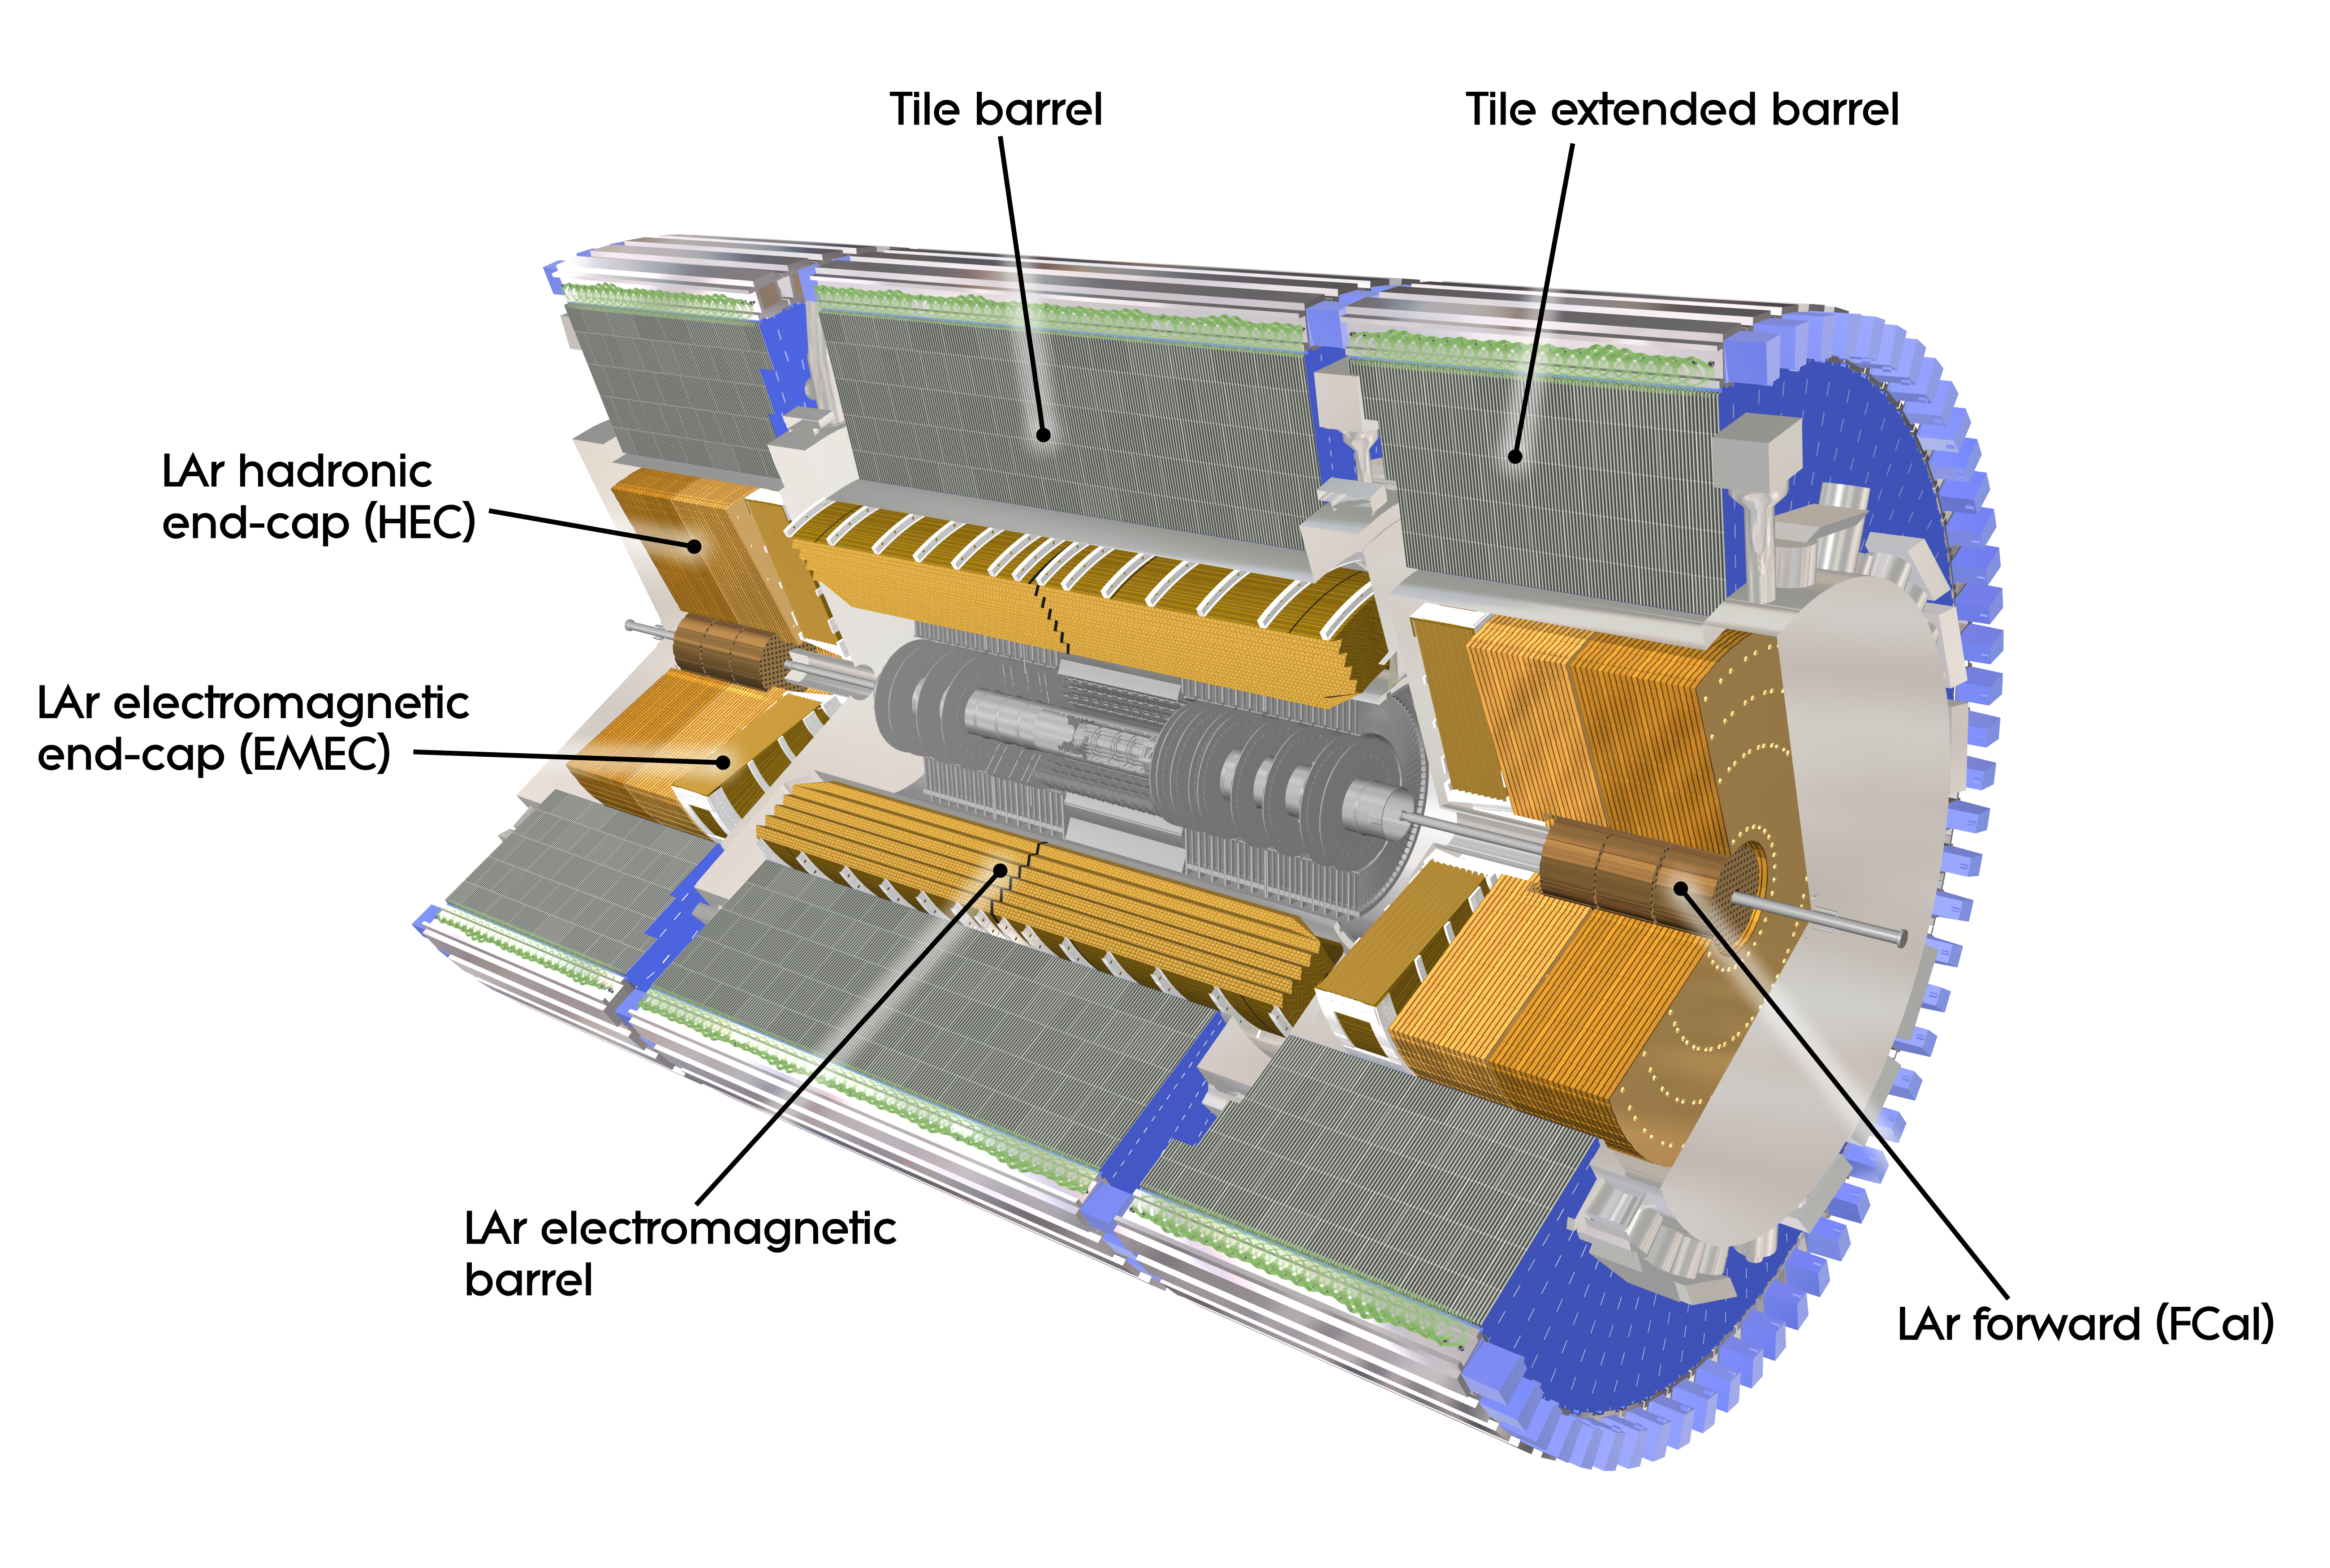
\includegraphics[width=\textwidth]{Detector/Calo/Calo-overview}
				\caption{A computer generated image of the full calorimeter.}
				\label{fig:Calo}
			\end{figure}

			The ATLAS Calorimeter system, shown in Figure~\ref{fig:Calo}, is comprised of two main sub-systems; the electromagnetic calorimeter (ECAL) and hadronic calorimeter (HCAL), which are designed to stop and measure the energy of electromagnetic-interacting and hadronic particles respectively. The combination of the two provides full coverage in $\phi$ and $\left | \eta \right | < 4.95$. Particles slow down and lose energy generating showers when crossing different layers. The ECAL is comprised of one barrel and two end-cap sectors employing liquid Argon (LAr). The showers hereby develop as electrons pairs which are then collected. The HCAL is also comprised of one barrel and two end-cap sectors. The sensors in the barrel of the HCAL are tiles of scintillating plastic whereas LAr is employed for the end-cap. A forward region, the closest possible to the beam, is covered by a LAr forward calorimeter (FCal). The LAr and Tile Calorimeter will be briefly discussed in the following parapgraphs. 
			%The particles have to deposit all their energy within the calorimeters to obtain an accurate energy measurement and avoid energy deposits in the outer muon spectrometer.
			%The definitions of radiation length ($X_0$), the distance over which an electron loses 1/$e$ of its energy within a given material, and nuclear interaction length ($\lambda_I$), are used to define the lengths of the barrel and the endcap regions of the calorimeter system. The ECAL roughly measures 22 $X_0$ thick in the region of barrel, and 24 $X_0$ in the end caps. The HCAL roughly measures 10 $\lambda_I$. Both ECAL and HCAL measures vary with $\eta$. Furthermore, it is known that hadronic particles are more penetrating than the electromagnetic ones and in particular, $\lambda_I$ is roughly ten times bigger than $X_0$. 

			\subsection*{The Liquid Argon Calorimeters}

 				The ECAL is comprised of multiple layers of liquid Argon (LAr) sampler and lead absorber. The choice of its accordion-geometry design brought two main advantages; full $\phi$ coverage with no non-interactive regions (no cracks); fast extraction of signals coming from both front or rear end of the electrodes. It is made of two half-barrel wheels, both placed in the barrel cryostat, that provide a pseudorapidity coverage up to $\left | \eta\right | < 1.475$ and two end-cap detectors providing $1.375 \leq \left|\eta\right| \leq 3.20$ coverage in two end-cap cryostats. The junction between the barrel and end cap components defines the crack region and any signal coming from the crack region is therefore discarded. 

 				In the $\left | \eta\right | < 1.8$ region there is an additional layer, placed at the front of the calorimeter, that is made of a thin (0.5 cm in the end-cap and 1.1 cm in the barrel) LAr layer with no absorber~\cite{ATLASLAR}. This additional layer was designed to correct for the energy lost, as particles enter the calorimeter, by taking a measurement just before the majority of the electomagnetic shower is developed.

 				% In the barrel, the accordion layers are axial and run in $\phi$, the folding angles of the layers vary with radius to keep the liquid-argon gap constant. 
 				% In the end-caps the layers are parallel to the radial direction and run axially. 
 				% The LAr is ionised by electromagnetic showers. The read-out circuits are made of three copper layers insulated by two layers of polyimide. 
 				% The two outer layers, split in sectors, are connected to high-voltage sources and polarize the LAr gap to the absorber. 
 				% The inner layer is where the signal is collected through capacitive coupling and is then segmented into read-out pads.

			\subsection*{The Tile calorimeter}

				The main purpose of the hadronic calorimeter is to measure the energy of hadronic showers. It is built employing steel and scintillating tiles coupled to optical fibres which are read out by photo-multipliers. As shown in Figure~\ref{fig:Calo}, the HCAL is made up of three cylinders; a central barrel, 5.64 m long covering a region $\left | \eta \right | < 1.0$, and two extended barrel, 2.91 m long covering a reigon $0.8 < \left | \eta \right | < 1.7$. Each cylinder is made up of 64 modules and each module is in turn made up of three layers. Ultimately, the smallest section of the calorimeter module is a cell with a $\Delta \phi \times \Delta \eta = 0.1 \times 0.1$ granularity for the two innermost layers and $\Delta \phi \times \Delta \eta = 0.2 \times 0.1$ for the outermost one. 

		% --------------------------------
		% -------  THE MU SPEC
		% --------------------------------
		\subsection{The Muon Spectrometer}
		\label{sec:MuSpec}

			The MS~\cite{MSTDR}, shown in Figure~\ref{fig:MS}, is the outermost sub-system of the whole ATLAS detector. As such, it surrounds the calorimeters and its main function is to perform precision measurement of muons momenta. The deflection of muon tracks employing large superconducting air-core toroid magnets and high-precision tracking chambers is at the heart of such high precision measurement. 

			\begin{figure}[!htb]
				\centering
				\includegraphics[width=\textwidth]{Detector/MS/MS}
				\caption{Cut-away view of the ATLAS muon system~\cite{ATLASJINST}.}
				\label{fig:MS}
			\end{figure}

			The MS is comprised of one large barrel toroid, covering the region $\left| \eta \right | \leq 1.4$, and two end-cap toroids, covering $1.6 < \left| \eta \right| \leq 2.7$ which are employed together to achieve the track-bending effect wanted. The magnitude of the magnetic field in the barrel, generated by eight large superconducting coils, ranges from 0.5 to 2 T. 

			Around the beam axis, three cylindrical layers make way for the chambers, placed in planes perpendicular to the beam, used to measure tracks. 

			Monitored Drift Chambers (MDTs) are employed over most of the pseudorapidity range to provide precision measurement of track coordinates in the bending direction. 
			Cathode Strip Chambers (CSCs) are instead employed at large pseudorapidity ($2 < \left | \eta \right | < 2.7$). 
			Finally, in the end-cap regions Thin-Gap Chambers (TGCs) together with Resistive-Plate Chambers (RPCs) are dedicated to the Trigger System discussed in Section~\ref{sec:trigSyst}. 


	% --------------------------------
	% -------  THE TRIGGER
	% --------------------------------
	\section{The ATLAS Trigger System}
	\label{sec:trigSyst}

		\begin{figure}[!htb]
			\centering
			\includegraphics[width=\textwidth]{Detector/Trigger/TDAQSystem}
			\caption{The ATLAS TDAQ system. L1Topo and FTK have not been used for the results shown in this thesis~\cite{ATLASTrigger2015}.}
			\label{fig:TDAQSyst}
		\end{figure}

		The ATLAS Trigger System is at the heart of data taking. It is an essential component of any nuclear or particle physics experiment since it is responsible for deciding whether or not to store an event for later study~\cite{ATLASTrigger2015}. Its main function to reduce the event rate from $\sim$ 40 MHz\footnote{The LHC delivers beams with a bunch-spacing of 25 ns.} bunch-crossing\footnote{The term bunch-crossing is hereby used when referring to a collision between two bunches of protons. Since only a certain fraction of the total momentum carried by each proton contributes to the collision, an average number of interactions per bunch-crossing, $\left < \mu \right >$ is used.} to $\sim$ 200 Hz which corresponds to roughly 300 MB/s.

		The Trigger and Data Acquisition (TDAQ) utilises a two-level system shown in Figure~\ref{fig:TDAQSyst}, a first hardware-based level trigger (L1) and a software-based high-level trigger (HLT). The L1 trigger decision is formed by the Central Trigger Processor (CTP), which receives inputs from the L1 calorimeter (L1Calo) and L1 muon (L1Muon) triggers. L1 is a hardware-based system that uses information from the calorimeter and muon subdetectors, and defines the so-called Regions of Interest (RoIs) within the detector to be investigated by the next level trigger, the HLT. Additionally, a Fast TracKer (FTK) system~\cite{FTKTDR} (not yet installed) will provide global ID track reconstruction at the L1 trigger rate using lookup tables stored in custom associative memory chips for the pattern recognition. The FPGA-based track fitter will perform a fast linear fit and the tracks are made available to the HLT. This system will allow the use of tracks at much higher event rates in the HLT than is currently affordable using CPU systems. However, the upgrade of the ATLAS trigger will not be discussed any further.

		The ATLAS trigger system will be further discussed in Chapter~\ref{ch:trigger}.
    \chapter{The ATLAS Trigger System}
\label{ch:trigger}
\epigraph{\emph{Software is a great combination between artistry and engineering.}}{Bill Gates}
%\epigraph{\emph{Engineering. Where the noble semiskilled labourers execute the vision of those who think and dream. Hello, Oompa-loompas of science.}}{Sheldon Cooper}

	The \ac{ATLAS} trigger system together with its performance will be presented in this chapter. A brief introduction of the reason behind the need of a trigger system, together with its implementation in \ac{ATLAS}, will be discussed in Section~\ref{sec:Trig_intro}. The \ac{L1} trigger and \ac{HLT} will be discussed in Sections~\ref{sec:L1} and~\ref{sec:HLT}, respectively. Finally, Section~\ref{sec:Trig_perf} will be dedicated to the performance of \ac{HLT} for low-\pt\ single-lepton, missing transverse energy, \met - as the most relevant trigger for the analysis discussed in Chapter~\ref{ch:stop_ana} -, and medium- and high-\pt\ \bj\ triggers. This has been part of the \textit{qualification task}\footnote{In order to become an \ac{ATLAS} author every active \ac{ATLAS} researcher should spend $50\%$ of their time (in their first year), moving to $30\%$ the year after.} of the author and the results were published in a paper in the European Physics Journal~\cite{ATLASTrigger2015}.


	\section{Overview}
	\label{sec:Trig_intro}

		More than 80 \ifb\ of \pp\ collisions were delivered in 2016 and 2017 by the \ac{LHC} and, due to storage space limitations, it is not feasible to save all the information about the collision after every bunch crossing. The \ac{ATLAS} Trigger System is indispensable to reduce the read-out rate to a sensible value without affecting the physics programme of \ac{ATLAS}, \eg\ discarding potentially interesting events. A multiple-level architecture is employed to allow the trigger enough time to identify interesting events, using both software- and hardware-based real-time algorithms. 

		Figure~\ref{fig:TDAQSyst} shows the \ac{TDAQ} system. This is comprised of both a hardware-based first-level trigger (\ac{L1}) and a software-based \ac{HLT}, as already mentioned in Section~\ref{sec:trigSyst}. The \ac{L1} trigger decision is formed by the \ac{CTP}, which receives inputs from the \ac{L1Calo} and \ac{L1Muon} triggers. Once the events pass the \ac{L1} selection, they are buffered in the \ac{ROS} and processed by the \ac{HLT}, which receives information on the \ac{RoI} from \ac{L1} to be used for track reconstruction in the trigger algorithms.
		%\footnote{A Region of Interest is an $\eta-\phi$ region within the \ac{ATLAS} detector identified by the \ac{L1} Trigger}
		An \ac{RoI} is an extended wedge-shaped spatial region in the detector, consisting of a direction in $\eta-\phi$ originating from a $z$-position along the beam-line, extended along the beam-line by independent directions with respect to this $z$ position, and extended about the $\phi$ direction with independent directions in pseudo-rapidity, at the maximum and minimum $z$ positions along the beam-line. %In other words, an RoI is not just a simple inverted pyramid with the apex on the beam-line, but a wedge extended along the beam-line, since the $z$ vertex position is not known until after the tracking has taken place, so the \ac{RoI} must be extended along the full length of the interaction region at the beam-line.	%%% ROI DEFINITION Events accepted by \ac{HLT} are then transferred to local storage and exported to the \emph{Tier-0} facility at CERN’s computing centre for offline reconstruction.

		\begin{figure}[!htb]
			\centering
			\includegraphics[width=\textwidth]{Detector/Trigger/TDAQSystem}
			\caption{The \ac{ATLAS} \ac{TDAQ} system. \acs{L1Topo} and \ac{FTK}~\cite{ATLASTrigger2015} have not been used for the results shown in this thesis.}
			\label{fig:TDAQSyst}
		\end{figure}

		The trigger system is configured via the so-called trigger \textit{menu}, which contains the multiplicity requirement (number of tracks) and the pre-scale factors\footnote{A factor associated with a trigger at each level that indicates what fraction of events, that could pass this trigger selection, is actually accepted.} for the selected events. Additionally, the menu is meant to define the trigger \textit{chains} - usually referred to just as trigger - that start from a \ac{L1} trigger and specify a sequence of reconstruction and selection steps for the specific trigger signatures required in the trigger chain. This is named after the following convention: 

		$$\mathrm{TriggerLevel\_TypeAndThreshold\_Identification\_Isolation}$$

		\noindent Here, ``TriggerLevel'' refers to either \ac{L1} or \ac{HLT}, ``TypeAndThreshold'' refers to the type of object to trigger on (electron, muon, \met, etc.) and its energy threshold. If any identification and/or isolation criteria are included, these are appended at the end of the name, \eg: \texttt{HLT\_e24\_lhmedium} is an electron trigger with a $24$ \GeV\ threshold, using ``medium'' identification criteria, which will be further discussed in Chapter~\ref{ch:evSimObjReco}. 
		% Figure~\ref{fig:trig_chain} shows an illustration of an electron-trigger chain used to select electrons \cite{ATLASTrigger2010}.

		% \begin{figure}
		% %\begin{wrapfigure}{L}{.5\textwidth}
		% 	\centering
		% 	%\includegraphics[height=.3\textheight]{Trigger/trig_chain}
		% 	\includegraphics[width=.3\textwidth]{Trigger/trig_chain}
		% 	\caption{\label{fig:trig_chain} An illustration of an Electron-trigger chain (from \cite{ATLASTrigger2010}).}
		% %\end{wrapfigure}
		% \end{figure}


		
	\section{Level-1 Trigger}
	\label{sec:L1}

		The \ac{L1} trigger decision is essentially taken by the \ac{CTP}, based on the information the \ac{L1} calorimeter and \ac{L1} muon trigger systems. Additionally, a \ac{L1Topo} trigger\footnote{Two FPGA-based (Field-Programmable Gate Arrays) processor modules}, fed with energy and direction information about the objects found by the \ac{L1Calo} and \ac{L1Muon} triggers, is employed~\cite{ATLASJINST,ATLASTrigger2015,ATLASL1Topo}.

		The \ac{L1} trigger system is implemented in fast custom electronics to keep the decision time around 2.5 $\mu$s and its decision is used as a \emph{seed} for \ac{HLT}. 


		\subsection*{The L1 Calorimeter Trigger}

			\begin{wrapfigure}{L}{.5\textwidth}
			%\begin{figure}[!htb]
				\centering
				\includegraphics[width=.4\textwidth]{Trigger/cluster}
				\caption{\label{fig:calo_cluster} Illustration of the electron/photon and tau algorithms with the sums to be compared to programmable thresholds (from \cite{ATLASTrigger2010}).}
			%\end{figure}
			\end{wrapfigure}

			The \ac{L1Calo} trigger~\cite{ATLASJINST, ATLASL1CaloTrig} is based on inputs from the electromagnetic and hadronic calorimeters within the region $\abseta<4.9$. It provides triggers for objects such as electrons/photons, taus, jets, and global transverse energy. Dedicated analogue trigger signals, provided by the \ac{ATLAS} calorimeters independently from the signals read out and used at the \ac{HLT} and offline, make the \ac{L1Calo} trigger decision, which is based on the information from analogue sums of calorimeter elements, called \emph{trigger towers}, instead of using the full granularity of the calorimeter. The trigger towers have a size of approximately $\Delta \eta \times \Delta \phi = 0.1$ in the central part of the calorimeter, $\abseta < 2.5$, and they get larger and less regular in the forward region. Separate trigger towers are employed for electromagnetic and hadronic calorimeters. Furthermore, two processor systems run the trigger algorithms, once the signals have been digitised: the first, called \emph{cluster processor}, uses the full \ac{L1} trigger granularity information in the central region to look for small and localised clusters, which are typical a energy deposit left by an electron, photon or tau; the second, the \emph{jet and energy-sum processor}, uses $2 \times 2$ sums of trigger towers (jet elements), to identify jet candidates and form missing transverse energy, \met, and total transverse energy, \et. As an example, Figure~\ref{fig:calo_cluster} shows a sketch of the electron/photon and tau triggers. The trigger algorithm identifies a Region of Interest as a $2 \times 2$ trigger tower cluster in the electromagnetic calorimeter for which the transverse-energy sum, released in at least one of the four possible pairs of nearest neighbour towers ($1 \times 2$ or $2 \times 1$), exceeds a pre-defined threshold. Additionally, jets \ac{RoI}s are defined as $4 \times 4$, $6 \times 6$ or $8 \times 8$ trigger-tower windows for which the summed electromagnetic and hadronic transverse energy exceeds pre-defined thresholds and which surround a $2 \times 2$ trigger tower core that is a local maximum that will be also used to define the coordinates of the jet \ac{RoI}.


		\subsection*{The L1 Muon Trigger}

			The \ac{L1Muon} trigger system~\cite{ATLASPerf08} processes input data from fast muon trigger sub-detectors and its main task is to select muon candidates with a \pt\ threshold of 6 \GeV\ and identify the bunch crossing in which they were produced.

			Figure~\ref{fig:L1MuTrig} shows how muons are triggered at \ac{L1}. The \ac{RPC} system in the barrel region ($\abseta < 1.05$) and the \ac{TGC} system in the end-cap regions ($1.05 < \abseta < 2.4$) are employed. They provide a rough measurements of muon-candidate \pt, $\eta$, and $\phi$. Three planes in the barrel and three in each endcap form the trigger chambers. Each plane is comprised of two to four layers and muon candidates are identified by forming coincidences between the muon planes. Coincidences are formed requiring hits that lie within parametrised geometrical muon \emph{roads}. A road, as the example shown in Figure~\ref{fig:L1MuTrig}, essentially contains the trajectories, from the interaction point, of either positively or negatively charged muons with a \pt\ above a given threshold. In particular six programmable \pt\ thresholds are employed at \ac{L1}, divided into two sets: three low-\pt\ thresholds meant to cover values up to 10 \GeV, and three high-\pt\ thresholds meant to cover $\pt > 10 \GeV$.

			\begin{figure}[!htb]
				\centering
				\includegraphics[width=\textwidth]{Trigger/L1MuTrigChambers}
				\caption{\label{fig:L1MuTrig} A schematic view of the \ac{L1Muon} trigger chambers (from \cite{ATLASTrigger2010}).}
			\end{figure}


		\subsection*{The CTP}

			The \ac{CTP}~\cite{ATLASJINST} applies the multiplicity requirements and pre-scale factors specified in the trigger menu to the inputs from the \ac{L1} trigger systems and forms the \ac{L1} trigger decision. Timing and control signals\footnote{The timing signals are defined with respect to the \ac{LHC} bunch crossings: a 25 ns time window centred on the instant at which a proton bunch might cross the \ac{ATLAS} interaction point.} are employed to distribute the \ac{L1} trigger decision to all \ac{ATLAS} sub-detector readout systems. The \ac{CTP} is responsible for applying the so-called \emph{preventive dead-time}, meant to limit the minimum time between two consecutive \ac{L1} accepts (\emph{simple dead-time}), $\mathcal{O}(100 \mathrm{ns})$, in order to both avoid overlapping readout windows, and restrict the number of \ac{L1} accepts allowed in a given number of bunch-crossings (\emph{complex dead-time}) to avoid buffers from overflowing. In addition, a \emph{busy dead-time}, can be introduced by \ac{ATLAS} sub-detectors to temporarily throttle the trigger rate. These dead-times are used to monitor the total \ac{L1} trigger rate, and individual trigger rates that need to be monitored before and after any pre-scales and/or any vetoes that have been applied. Furthermore, such information is also used to provide a measure of the \ac{L1} dead-time, which has to be accounted for when determining the luminosity~\cite{ATLASTrigger2010}.

		

			


	\section{High-Level Trigger}
	\label{sec:HLT}

		The events that are accepted by \ac{L1} are then buffered in the \ac{ROS} and processed by the \emph{High-Level Trigger} using information that is not available at \ac{L1}, such as finer-granularity calorimeter inputs, precision measurements from the \ac{MS} and tracking information from the \ac{ID}. \ac{HLT} receives \ac{RoI} from \ac{L1} and performs the reconstruction within them. As needed, the reconstruction performed by the \ac{HLT} software can either be run within \ac{RoI}s or performing a so-called \emph{full scan} of the detector. In order to reduce the processing time, a two-stage approach is employed for most \ac{HLT} triggers: a first reconstruction (fast) to reject the majority of events; a second precision reconstruction for the remaining events (slower). Events that are accepted by the \ac{HLT} get transferred to local storage at the experimental site and exported to the \ac{CERN}’s computing centre for offline reconstruction~\cite{ATLASTrigger2015}. 

		
		\subsection{Inner detector tracking}
		\label{sec:tracking}

			The track reconstruction in the Inner Detector is a vital component of the trigger decision in the \ac{HLT}. A robust reconstruction of particle trajectories is an essential prerequisite for triggering on electrons, muons, taus, and $b$-jets. Furthermore, it is also used for triggering on inclusive \pp\ interactions and for the on-line determination of the beam spot\footnote{The luminous region produced by the collisions of proton beams.} where the reconstructed tracks provide the input for vertex reconstruction.

			The ID tracking in the trigger also includes information from the IBL, which significantly improves the tracking performance and in particular the impact parameter resolution~\cite{IBLTDR}. The tracking algorithms are called \emph{Fast Tracking} and \emph{Precision Tracking}. The former is comprised of trigger-specific pattern recognition algorithms, unlike the latter which is heavily based on offline-tracking algorithms.
			As already mentioned, once an \ac{RoI} has been identified by \ac{L1}, the algorithms are typically configured to run within it. Furthermore, in order to reduce \ac{CPU} usage, the offline track-finding is seeded with tracks and space-points identified by fast tracking stage seeds. The running of the full \ac{HLT} reconstruction for each event on an individual node allows for the two stages of the trigger, \eg\ $b$-jet triggers, which will be discussed in Section~\ref{sec:Trig_perf}, to share the data preparation so detector information only needs to be read out once. 
			% Running the full \ac{HLT} reconstruction for each event on an individual node, affords the opportunity to better optimise the \ac{RoI} geometry and use an advanced multi-stage strategy for the tau and $b$-jet triggers, which will be discussed in Section~\ref{sec:Trig_perf}. 

			In order to reduce the detector volume of \ac{RoI}, an advanced multi-stage approach, in particular for tau and \bj\ tracking, is employed. The first stage is to identify leading tracks within an \ac{RoI}, long in $z$ but narrow in $\eta$ and $\phi$, by running the \ac{FTF} algorithm. The leading tracks are used to construct a second-stage \ac{RoI}, constrained in both $\eta$ and $\phi$, but very tightly constrained in polar angle and with a small $z$ position width. The \ac{FTF} is then run again within the wider second-stage \ac{RoI}, followed by the Precision Tracking~\cite{ATLASTrigger2015, Miano:2016oty}. The second stage, the Precision Tracking, is heavily based on an optimised subset of the tracking algorithms used offline, which is slower than the first but, in return, it identifies objects constructed starting from the inner detector tracks.

			%As the future inclusion of the FTK tracks had to be taken into account, tracks provided by the FTK were integrated into the system although they were not used for any of the results presented in this work. 


		\subsection{Performance of HLT}
		\label{sec:Trig_perf}

			The performance of the tracking was estimated using 13-\TeV\ \pp\ collision events collected in July 2015 by the \ac{ATLAS} detector (unless otherwise stated). In order to be as unbiased as possible, specific monitoring triggers that do not require a track to be present for the event to be accepted are used to estimate the efficiency of the tracking algorithms. All the quantities used to estimate the performance of the tracking, \ie\ efficiencies, residuals and resolutions, are calculated with respect to the tracks found by the offline reconstruction software. In particular, the efficiency is defined as the fraction of offline reference tracks that are matched to a trigger track 

			\begin{equation}
				\mathcal{E} = \frac{N_{\mathrm{trigger}}}{N_{\mathrm{offline}}}
				\label{eq:trig_eff}
			\end{equation}

			The tracking efficiency has been estimated for electrons and muons for the single-stage tracking, and for $b$-jets for the multi-stage approach, as part of the author's qualification task. The reconstructed tracks are required to have at least two (six) Pixel (\ac{SCT}) clusters and lie within the region $\abseta < 2.5$. The closest trigger track within a cone of size $\Delta R =  \Delta \eta^2 + \Delta \phi^2 = 0.05$ of the offline reconstructed track is selected as the matching trigger track.


			\subsubsection*{Electrons}

				Figure~\ref{fig:ele_idtrig_eff} shows the tracking efficiency for the 24 GeV electron trigger as a function of $\eta$ and \pt\ of the offline track. The tracking efficiency is measured with respect to offline tracks with $\pt > 20$ \GeV\ for tight offline electron candidates from the 24 GeV electron support trigger, which does not use the trigger tracks in the selection, despite being identical to the physics trigger. The \ac{FTF} and Precision Tracking efficiencies are all above 99\% within the whole pseudo-rapidity range. The small efficiency drop at low \pt\ is due to bremsstrahlung energy loss by electrons~\cite{ATLASTrigger2015}.

				\begin{figure}[!htb]
					\begin{center}
						\subbottom[]{
							\includegraphics[width=0.45\textwidth]{Trigger/id/elec24plots3fb160224/HLT_eta_eff.pdf}}\hspace{0.05\textwidth}
						\subbottom[]{
							\includegraphics[width=0.45\textwidth]{Trigger/id/elec24plots3fb160224/HLT_pT_eff.pdf}}\hspace{0.05\textwidth}
					\end{center}
					\caption{The ID tracking efficiency for the 24 \GeV\ electron trigger is shown as a function of the (a) $\eta$ and (b) $\pt$ of the track of the offline electron candidate. Uncertainties based on Bayesian statistics are shown (from~\cite{ATLASTrigger2015}).}
					\label{fig:ele_idtrig_eff}
				\end{figure}


			\subsubsection*{Muons}

				Figure~\ref{fig:idmuontriggera} shows the muon tracking performance with respect to offline muon candidates with $\pt > 6 \GeV$ selected by the 6 \GeV\ muon support trigger as a function of the offline muon \pt. The efficiency is well above 99\% in the entire \pt\ range for both \ac{FTF} and Precision Tracking. Figure~\ref{fig:idmuontriggerb} shows the resolution of the transverse track impact parameter with respect to offline as a function of the offline muon \pt. \ac{FTF} and Precision Tracking resolutions are better than 17 and 15 $\mu$m, respectively, for muon candidates with offline $\pt > 20 \GeV$. The difference ($\sim 10\%$) between the two algorithms is driven by the fact that Precision Tracking (black solid points) uses the space points found by the \ac{FTF} (red open points), but refits them using the offline algorithm. In other words, Precision Tracking runs a faster version of the full offline track fit and it performs better.

				\begin{figure}[!htb]
					\begin{center}
						\subbottom[]{
						  \includegraphics[width=0.45\textwidth]{Trigger/id/mu6plots3fb/HLT_pT_eff.pdf}\label{fig:idmuontriggera}}\hspace{0.05\textwidth}
						\subbottom[]{
						  \includegraphics[width=0.45\textwidth]{Trigger/id/mu6plots3fb/HLT_rd0_vs_pt_sigma.pdf}\label{fig:idmuontriggerb}}
					\end{center}
					\caption{ 
					The ID tracking performance for the 6 \GeV\ muon trigger;
					(a) efficiency as a function of the offline reconstructed muon \pt,  
					(b) the resolution of the transverse impact parameter, $d_{0}$  as a function of the offline reconstructed muon \pt. Uncertainties based on Bayesian statistics are shown (from~\cite{ATLASTrigger2015}).}
					\label{fig:idmuontrigger}
				\end{figure}



			\subsubsection*{\emph{b}-jets}

				As previously mentioned, the $b$-jet triggers tracking algorithms are run in a larger \ac{RoI} than for electrons or muons and in order to limit \ac{CPU} usage, multiple stage track reconstruction was implemented and deployed during Run-2.

				First, the leading track and its position along the beam-line are determined by executing fast tracking in an \ac{RoI} that is fully extended along the beam-line, in the $|z|<225$ mm region, but narrow (0.1) in both $\eta$ and $\phi$, as shown in the blue-shaded region in Figure~\ref{fig:idroi}. The second stage is then run, using this position along the beam-line, to reconstruct all tracks in an \ac{RoI} that is larger (0.4) in both $\eta$ and $\phi$ but limited to $|\Delta z|<10$ mm with respect to the leading track, as shown by the green-shaded region in Figure~\ref{fig:idroi}.

				\begin{figure}[!htb]
					\centering
					\includegraphics[width=0.65\textwidth]{Trigger/id/roi-plan}
					\includegraphics[width=0.3\textwidth]{Trigger/id/roi}
					\caption{An illustration of the \ac{RoI}s from the single-stage and two-stage tau lepton trigger tracking, shown in plan view (x-z plane) along the transverse direction and in perspective view. The z-axis is along the beam line. The combined tracking volume of the $1^{\mathrm{st}}$ and $2^{\mathrm{nd}}$ stage \ac{RoI} in the two-stage tracking approach is significantly smaller than the \ac{RoI} in the one-stage tracking scheme (from~\cite{ATLASTrigger2015}).}
					\label{fig:idroi}
				\end{figure}

				The first-stage vertex tracking takes all jets identified by the jet trigger with $\eta > 30$ \GeV\ and reconstructs tracks with the \ac{FTF} in a narrow region in $\eta$ and $\phi$ around the jet axis for each jet, but with $|z|<225$ mm along the beam line.
				
				Following this step, the primary vertex reconstruction~\cite{ATLAS-CONF-2010-069} is performed using the tracks from the fast tracking stage. This vertex is used to define wider \ac{RoI}s around
				the jet axes, with $|\Delta\eta|<0.4$ and $|\Delta\phi|<0.4$ but with $|\Delta z|<20$ mm relative to the primary vertex $z$ position. These \ac{RoI}s are then used for the second-stage 
				reconstruction that runs the fast track finder in the wider $\eta$ and $\phi$ regions followed by the Precision Tracking, secondary vertexing and $b$-tagging algorithms, which will not be discussed in this work.

				The performance of the primary vertexing in the $b$-jet vertex tracking can be seen in Figure~\ref{fig:bjetvertexa}, which shows the vertex finding efficiency with respect to 
				offline vertices in jet events with at least one jet with transverse energy above 55, 110, or 260 \GeV\ and with no additional $b$-tagging requirement. The efficiency is shown 
				as a function of the number of offline tracks with $\pt>1 \GeV$ that lie within the boundary of the wider \ac{RoI} (defined above) from the selected jets. The efficiency rises sharply and 
				is above 90\% for vertices with three or more tracks, and rises to more than 99.5\% for vertices with five or more tracks. The resolution in $z$ with respect to the offline $z$ position as shown in Figure~\ref{fig:bjetvertexb} is better than 100 $\mu$m for vertices with two or more offline tracks and improves to 60 $\mu$m for vertices with ten or more offline tracks.

				\begin{figure}[!htb]
					\begin{center}
						\subbottom[]{
							\includegraphics[width=0.45\textwidth]{Trigger/id/bjetvtx/HLT_xPrimVx_ntrax_eff.pdf}\label{fig:bjetvertexa}}\hspace{0.05\textwidth}
						\subbottom[]{
							\includegraphics[width=0.45\textwidth]{Trigger/id/bjetvtx/HLT_xPrimVx_rdz_vs_ntrax_sigma.pdf}\label{fig:bjetvertexb}}
					\end{center}
					\caption{The trigger performance for primary vertices in the $b$-jet signatures for 55, 110 and 260 \GeV\ jet triggers; (a) the vertexing efficiency as a function of the number of offline tracks within the jets used for the vertex tracking, (b) the resolution in $z$ of the vertex with respect to the offline vertex position as a function of the number of offline tracks from the offline vertex (from~\cite{ATLASTrigger2015}).}
					\label{fig:bjetvertex}
				\end{figure}

			\subsubsection*{Missing Transverse Energy, \met}

				There exists several algorithms to reconstruct the \met\ at the \ac{HLT}. The \textit{missing} \HT\footnote{\HT\ is the scalar sum of the various \pt s in the event, $\displaystyle \HT = \sum_{i} \pt^i$.} (MHT) algorithm calculates \met\ as the negative sum of transverse energy of calibrated jets, constructed from calibrated topological clusters of calorimeter cells. This algorithm is the most relevant to the analysis presented in Chapter~\ref{ch:stop_ana}. The \textit{cell algorithm} is based on the negative sum of transverse energy deposited in calorimeter cells above a certain noise threshold. Unlike the cell algorithm, which calculates \met\ on the electromagnetic scale, the MHT algorithm looks at jets calibrated using jet energy scale, so that numerical threshold values for similar signal efficiencies differ. \textit{Pufit}, a third algorithm, was employed to disentangle calorimeter deposits from the hard-scatter, from those originating from pile-up interactions by grouping towers made out of topological clusters into a pile-up and a hard-scatter category. This grouping is based on their energy, where the threshold itself is dependent on the overall event activity measured by the total energy deposited in the calorimeter. The assumption is that the contribution to \met\ due to pile-up interactions is zero. Nevertheless a minimisation, which takes into account resolution terms, determines an effective energy density from pile-up interaction which allows a vanishing contribution to \met\ by the pile-up calorimeter towers. This correction is then subtracted from the hard-scatter towers. The negative sum of transverse energy of those pile-up corrected hard-scatter towers will provide the final \met\ value~\cite{ATL-COM-DAQ-2016-137}.

				Figure~\ref{fig:mettrigger} shows the turn-on curves for various \met\ triggers: Figure~\ref{fig:mettriggera} shows the efficiency as a function of \textit{modified}\footnote{To calculate the \met\ efficiency, \eg\ in events with muons, a muon trigger must be employed, therefore muon contributions are removed.} offline \met\ for three different \met\ trigger algorithms, using early 2016 \pp\ collision data. The events have been selected using single lepton (electron or muon) triggers. The x-axis shows the offline \met\ calculated from the sum of electrons, photons and jets, without the contributions from the muons. Three different \met\ high-level trigger algorithms are shown: \texttt{HLT\_xe80\_tc\_lcw\_L1XE50} calculates \met\ based on calibrated clusters of calorimeter cells, and has a threshold of 80 \GeV. \texttt{HLT\_xe90\_mht\_L1XE50} calculates \met\ based on reconstructed jets, and it has a threshold of 90 GeV. \texttt{HLT\_xe100\_L1XE50} calculates \met\ based on calorimeter cells calibrated at the electromagnetic scale, and has a threshold of 100 \GeV. All three algorithms are seeded by a Level-1 trigger with a threshold of 50 \GeV\ which is also shown; Figure~\ref{fig:mettriggerb} shows the combined \ac{L1} and \ac{HLT} efficiency of the missing transverse energy triggers \texttt{HLT\_xe110\_pufit\_L1XE50} and \\ \texttt{HLT\_xe110\_mht\_L1XE50} as well as the efficiency of the corresponding \ac{L1} trigger (L1\_XE50) are shown as a function of the reconstructed \met\ (modified to count muons as invisible) using \pp\ collision data collected in 2017. The events shown are taken from data with a $\Wboson \to \ell \nu$ selection to provide a sample enriched in real \met. The \ac{HLT} \met\ of the \textit{pufit} algorithm is calculated as the negative of the transverse momentum vector sum of all calorimeter topological clusters corrected for pile-up. The pile-up correction is done by grouping the clusters into coarser “towers” which are then marked as pile-up if their $E_\mathrm{T}$ falls below a pile-up-dependent threshold.

				\begin{figure}[!htb]
					\begin{center}
						\subbottom[]{
							\includegraphics[width=0.45\textwidth]{Trigger/hlt_met_unprescaled2016.png}\label{fig:mettriggera}}\hspace{0.05\textwidth}
						\subbottom[]{
						  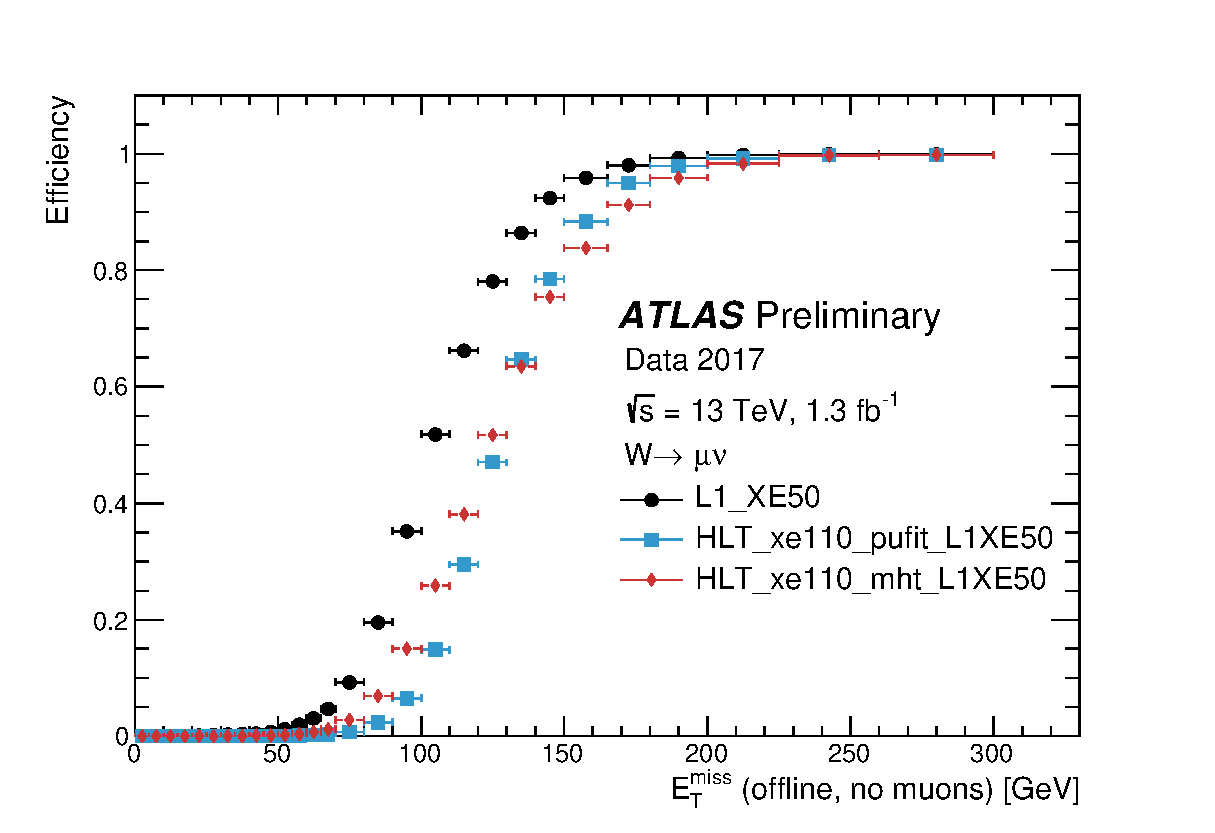
\includegraphics[width=0.45\textwidth]{Trigger/hlt_met_unprescaled2017.eps}\label{fig:mettriggerb}}
					\end{center}
					\caption{Turn-on curves of various \met\ triggers: Figure~\ref{fig:mettriggera} shows the efficiency as a function of offline \met\ for three different \met\ trigger algorithms. Three different \met\ high-level trigger algorithms are shown: \texttt{HLT\_xe80\_tc\_lcw\_L1XE50} calculates \met\ based on calibrated clusters of calorimeter cells, and has a nominal threshold of 80 \GeV. \texttt{HLT\_xe90\_mht\_L1XE50} calculates \met\ based on reconstructed jets, and has a nominal threshold of 90 \GeV. \texttt{HLT\_xe100\_L1XE50} calculates \met\ based on calorimeter cells calibrated at the electromagnetic scale, and has a nominal threshold (at the electromagnetic scale) of 100 \GeV. All three algorithms are seeded by a Level-1 trigger algorithm with a nominal threshold of 50 \GeV\ which is also shown; Figure~\ref{fig:mettriggerb} shows missing transverse energy trigger efficiencies for \texttt{HLT\_xe110\_pufit\_L1XE50} and \texttt{HLT\_xe110\_mht\_L1XE50} and for the corresponding \ac{L1} seed (\texttt{L1\_XE50}). (from~\cite{ATLASMETTriggerPublicPage}).}
					\label{fig:mettrigger}
				\end{figure}

    \chapter{Event Simulation and Reconstruction}

	bla bla bla 

	\section{Event Generation}

			bla bla

		\subsection{Parton Distribution Functions (PDFs)}

			bla bla bla 

		\subsection{Matrix Element Calculation}

			bla bla bla 


		\subsection{Parton Showers}

			bla bla bla 


		\subsection{Hadronisation}

			bla bla bla 



	\section{Detector Simulation}
		bla bla bla 




	% \section{Reconstruction}

	% 	\subsection{Pile-up in the Inner Detector}


	% 	\subsection{Tracks}


	% 	\subsection{Vertex}


	% 	\subsection{Electrons}


	% 	\subsection{Muons}


	% 	\subsection{Jets}


	% 	\subsection{Taus}


	% 	\subsection{Missing Transverse Energy}




	% \section{Object Selection}

	% 	\subsection{Baseline Leptons}


	% 	\subsection{Baseline Jets}


	% 	\subsection{Baseline Taus}


	% 	\subsection{Overlap Removal}


	% 	\subsection{Signal Leptons}


	% 	\subsection{Signal Jets}


	% 	\subsection{Signal Taus}




	% \section{Monte Carlo Samples}

	% 	\subsection{Generators}

	% 	\subsection{SM Background MC Samples}

	% 	\subsection{MC Signal Sample}




    \chapter[Search for top squarks in all-hadronic final states]{Search for top squarks in all-hadronic final states}
\label{ch:stop_ana}
\epigraph{\emph{In God we trust. All others must bring data.}}{William E. Deming}

	In this chapter the core of this thesis will be presented, namely the search for the direct pair-production of the supersymmetric partner of the top quark in all-hadronic final states using \pp\ collisions, at a centre-of-mass energy $\rts = 13$ \TeV, delivered by the \ac{LHC} and collected by the \ac{ATLAS} detector. A dataset of $36.1\, \ifb$ was used. Such measured value of integrated luminosity has an uncertainty of 3.2\% based on studies of scans of the $x-y$ beam separation carried out on both $2015$ and $2016$ datasets, where the average pileup parameter $\mu$ was $13.7$ and $24.9$, respectively.
		
	The results produced were published in a paper in the Journal of High Energy Physics in September 2017~\cite{stop0L}. A previous version of the analysis was also made public, using $13.3\,\ifb$ collected at $\rts = 13$ \TeV, with an earlier subset of the whole $2015+2016$ dataset, documented in an ATLAS conference note~\cite{ICHEPstop0L}. Although both versions contain author's contributions, only the results of the most recent analysis will be hereby discussed, as it represents the most updated, improved and extended version. Specifically, the optimisation of the search strategy, as well as the data-driven estimation of the number of events in the search regions for one of the most important backgrounds, and the evaluation of the related theory uncertainties, characterised the author's contributions. In addition, exception made for the optimisation strategy, the same contributions were also used in a different \ac{SUSY} analysis published in October 2017 in~\cite{DMhf}. Further details can be found in Appendix~\ref{ch:appA}.

	The chapter will be structured as it follows: an excursus on the simplified \ac{SUSY} models considered will be presented in Section~\ref{sec:susysig}; the selection of the events and the objects used in both data and \ac{MC} will be presented in Section~\ref{sec:evtsel}; the variables used and the optimisation of the regions in which the \ac{SUSY} signals were searched for will be presented in Section~\ref{sec:SRs}; the nominal procedure used  for the background estimation will be discussed in Section~\ref{sec:bkgest}, with particular focus on the data-driven background estimation in Section~\ref{sec:ddbkgest}; the results, together with their interpretation, will finally be presented in Section~\ref{sec:results}.


	\section{SUSY Signals}
	\label{sec:susysig}

		As already introduced in Section~\ref{sec:SUSYPheno}, the signals considered in this work are generated using simplified models, meaning that only the \stop, the \ninoone, the \ninotwo, and the \chinoonepm, were the \ac{SUSY} particles considered. In particular, in such considered models, either \ninotwo\ or \chinoonepm\ is assumed to be the \ac{NLSP} and, the chargino-neutralino mass splitting $\Delta m(\chinoonepm, \ninoone)$ is assumed to be $1$ \GeV, in accordance with the naturalness argument. This implies that the \chinoonepm\ will promptly decay to $\Wboson^*\ninoone$ , with the \Wboson\ emitted as a virtual particle. The decay products of the so-created virtual \Wboson\ will therefore be low \pt\ objects which will not be reconstructed by the \ac{ATLAS} detector. 

		\subsection{Benchmark processes}

			\begin{figure}[!htb]
				% \begin{center}
				\centering
					\subbottom[$\stop\ra t^{(*)}\ninoone$]{
						\includegraphics[width=0.25\textwidth]{theory/stst-bqqbqqN1N1-tt}}\hspace{0.05\textwidth}
					\subbottom[$\stop\ra b\ \chinoonepm\ra b \Wboson^{(*)}\ninoone$]{
						\includegraphics[width=0.25\textwidth]{theory/stst-bbWWN1N1}}\hspace{0.05\textwidth}
					\subbottom[$\stop\ra t\ \ninotwo\to h/Z\ \ninoone$]{
						\includegraphics[width=0.25\textwidth]{theory/stst-tbhWN1N1}}\hspace{0.05\textwidth}
				% \end{center}
				\caption{Diagrams of the decay topologies of the signal models considered in this work.}
				\label{fig:stopModels}
			\end{figure}

			Figure~\ref{fig:stopModels}(a)$-$(c) shows the diagrams corresponding to the decay scenarios considered in this work. In particular, (a) where both top squarks decay\footnote{The symbol (*) indicates off-shell production} via $\stop\rightarrow t^{(*)}\ \ninoone$; (b) where at least one of the stops decays via $\stop\rightarrow b\ \chinoonepm \rightarrow b\ \Wboson^{(*)}\ \ninoone$; (c) where $m_{\ninotwo}$ is small enough to allow one stop to decay via $\stop\to t\ \ninotwo \to h/Z\ \ninoone$ where $h$ is the \ac{SM} Higgs boson;

			\begin{wrapfigure}{R}{.5\textwidth}
				\centering\includegraphics[width=.25\textwidth]{theory/gogo-tsofttsoftN1N1-stst}
				\caption{Diagram of the gluino-mediated top squark production. The term ``soft" refers to decay products whose transverse momenta are below the detector thresholds.}
				\label{fig:gtt}
			\end{wrapfigure}

			The results were interpreted in the simplified models where only one- and two-step decays scenarios are allowed and, as already mentioned, the latter will be referred to as a natural \ac{SUSY}-inspired mixed grid, \ie\ $\Delta m(\chinoonepm, \ninoone) = 1 \GeV$~\cite{Alwall:2008ve, Alwall:2008ag, Alves:2011wf}. Furthermore, in both scenarios the \ac{LSP} is considered to be a pure bino state. The results will also be interpreted in two slices of the \ac{pMSSM} models: wino-\ac{NLSP} and well-tempered neutralino \ac{pMSSM}~\cite{Djouadi:1998di, Berger:2008cq}.
			A fourth scenario, in addition to direct pair production, was considered: top squarks can also be indirectly produced via gluino decays, as illustrated in Figure~\ref{fig:gtt}. In such model, the mass difference between the top squark and the neutralino is considered to be relatively small, $\Delta m(\stopone, \ninoone) = 5$ \GeV, allowing the jets originating from \stopone\ decay to have a \pt\ below the reconstruction threshold of the \ac{ATLAS} detector resulting in an experimental signature nearly equivalent to the one in Figure~\ref{fig:stopModels}(a).


		\subsection{MC samples}

			A grid of points across the $(\mstopone-\mninoone)$ plane with a $50$-\GeV\ spacing is generated to simulate the above-mentioned simplified models. %The mixing between the partners of the left- and right-handed top quarks is assumed to be maximal, \ie\ ..
			The signal models were generated using \texttt{MG5\_aMC@NLO 2.2-2.4}~\cite{madgraph} interfaced to \texttt{PYTHIA8}~\cite{pythia8} for the \ac{PS} and hadronisation. \texttt{EvtGen 1.2.0}~\cite{evtGen} was employed for the decays of the  $b$- and $c$-hadrons. The tree-level \ac{ME} calculation includes the emission of up to two additional partons for all signal samples. The \texttt{NNPDF2.3LO} \ac{PDF}~\cite{PDFs} set was used to generate the signal samples with the \texttt{A14}~\cite{CT10} tune for the \ac{UE} and shower parameters. Additionally, the CKKW-L prescription~\cite{CKKW} was used for the \ac{ME}–\ac{PS} matching. 

			The various signal cross sections were all calculated to next-to-leading order in the strong coupling constant, with the addition of soft-gluon emission re-summation at next-to-leading-logarithm accuracy (NLO+NLL)~\cite{Beenakker:1997ut, Beenakker:2010nq, Beenakker:2011fu}. The sparticle mass spectra for \ac{pMSSM} models were calculated using \texttt{Softsusy 3.7.3}~\cite{Allanach:2001kg, Allanach:2013kza} while the decays of each sparticle were performed by \texttt{HDECAY 3.4}~\cite{hdecay} and \texttt{SDECAY 1.5/1.5a}~\cite{sdecay}. Finally, various \ac{PDF} sets, factorisation, and re-normalisation scales were used to generate an envelope of cross-section predictions, within which a nominal value and uncertainty were chosen. Further details can be found in~\cite{Borschensky:2014cia}.



	\section{Objects definition}
	\label{sec:obj_def}
			
		The physics objects, as output of the reconstruction algorithms discussed in Section~\ref{sec:objReco}, are required to pass a first loose selection to be categorised as \emph{baseline} objects. An additional procedure is employed, to remove potentially overlapping objects, \eg\ a lepton is identified as a jet, or a lepton that falls within the same jet cone. The so-called \ac{OR} procedure, whose inputs are two baseline objects, is employed to resolve such ambiguity by discarding on of the two objects by looking at their $\Delta R$ as shown in Table~\ref{tab:OR}. 

		\begin{table}[!htb]\centering\caption{List of the possible ambiguities with relative criteria and decisions.}
			\begin{tabular}{cccc}
				\toprule 
				\textbf{Ambiguity} & \textbf{Criterion} & \textbf{Object kept} & \textbf{Object removed}\\
				\toprule
				\multirow{2}{*}{electron/jet} & $\Delta R (e,\mathrm{jet}) < 0.2$ & electron & jet\\
				& $0.2 \leq \Delta R (e,\mathrm{jet}) < 0.4$ & jet & electron \\\midrule
				electron/\bj & $\Delta R (e,\bj) < 0.2$ & \bj\ & electron\\ \midrule
				\multirow{2}{*}{muon/jet} & $\Delta R (\mu,\mathrm{jet}) < 0.4$ and & \multirow{2}{*}{muon} & \multirow{2}{*}{jet} \\ 
						& $N_{\mathrm{tracks}} < 3$, $\pt^{\mathrm{track}} > 500$ \MeV &  &  \\ \midrule
				photon/electron & $\Delta R (e,\gamma) < 0.4$ & electron & photon\\ 
				photon/muon & $\Delta R (\mu,\gamma) < 0.4$ & muon & photon\\ 
				photon/jet & $\Delta R (\mathrm{jet}, \gamma) < 0.4$ & jet & photon\\ 
				\bottomrule
				\end{tabular}
				\label{tab:OR}
		\end{table}

		The data-driven estimation of \ttZ\ events using \ttgamma\ is the only part of the analysis that used reconstructed photons. In particular, the \ac{OR} is modified accordingly to avoid that an object will appear in multiple collections (double-counting). The various baseline and signal objects can now be defined as it follows:

		\begin{description}
			\item[Electrons] 
				baseline electrons are required to have $\abseta < 2.47$, $\pT > 7$ \GeV\ and have to pass a variant of the \texttt{VeryLoose} likelihood-based selection (further details in~\cite{egamma, egamma2}). Electron candidates which pass the \ac{OR}, have a $\pt > 20$ \gev\ ($\pt > 28$ \GeV) in regions with a \met\ (lepton) trigger, satisfy $d_0/\sigma_{d_{0}} < 5$, $z_0 \sin \theta < 0.5$, and pass a \texttt{Tight} likelihood-based selection isolation, are tagged as signal;

			\item[Muons] 	
				baseline muons have to pass a \texttt{Loose} selection~\cite{PERF-2015-10}, satisfy $\abseta < 2.7$ and $\pt > 6$ \GeV. Further requirements are imposed on muon candidates to tag them as signal. In particular, they have to pass the \ac{OR}, a \texttt{Medium} quality selection~\cite{PERF-2015-10}, and satisfy
				$|d_0|< 3 \sigma_{d_0}$ and $|z_0 \times \sin \theta |<0.5$. Additionally, the \pt\ requirement is tightened up to $20$ \gev\ ($28$ \GeV) in regions with a \met\ (lepton) trigger;

			\item[Photons]
				baseline photons have to pass a \texttt{Tight}~\cite{Aaboud:2016yuq} selection, and have $\pt > 25$ \GeV\ and $\abseta < 2.37$. Additionally, baseline photon candidates are required to have $\pt > 130$ \GeV\ and satisfy a tighter isolation selection, in order to be tagged as signal;
			
			\item[Jets]
				as already mentioned in Chapter~\ref{sec:objReco}, jets are reconstructed using the \antikt\ algorithm with $R=0.4$. Baseline jets are required to have $\pt>20$ \GeV\ and $\abseta< 4.8$. Signal jets have to pass the \ac{OR}, satisfy the \ac{JVT} requirement, and have $\abseta < 2.8$ and $\pt > 20$ \GeV. 

			\item[b-tagged jets]
				baseline jets in the event are identified as originating from the decay of a $b$-quark is based on the \texttt{MV2c10} jet tagger which uses the a $77\%$ fixed-cut WP. The \pt\ threshold applied to signal jets is also applied to \bj\ and the requirement on the pseudorapidity is relaxed down to $\abseta < 2.5$.
			
			\item[Missing transverse energy]
				The \met\ is reconstructed as described in Section~\ref{sec:objReco}. Baseline muons, electrons, and jets after overlap removal are used in the \met\ recalculation. 
				% The \textit{soft} term in the event, already introduced in Section~\ref{sec:objReco}, that is not associated with any of the selected objects is calculated from inner detector tracks with $\pt > 400$ \MeV\ matched to the \ac{PV} to make it more resilient to pileup contaminations. 

				Additionally, in the analysis carried out during Run-1~\cite{Atlas8TeV} another \met-related quantity was introduced. The track-based \met, derived from the sum of the \pt\ of the tracks associated with the objects in the event was found to have discriminating power to reject fake \met. The \ptmisstrk, whose magnitude is \mettrk, from the tracking system is computed using the vector sum of the reconstructed inner detector tracks, $\ptmisstrk = \sum_i^{\mathrm{tracks}} \pt^i$, with $\pT > 500$ \MeV\ and $\abseta < 2.5$, that are associated with the \ac{PV} in the event. 
 		\end{description}

		Ultimately, leptons are also required to satisfy \pt-dependent track- and calorimeter-based isolation criteria. The calorimeter-based isolation is determined by taking the ratio of the sum of energy deposits in a cone of $R = 0.2$ around the electron or muon candidate and the energy deposits associated with the electron and muon. The track-based isolation is estimated in a similar way but using a variable cone size with a maximum value of $R = 0.2$ for electrons and $R = 0.3$ for muons. An isolation requirement is made that is $95\%$ efficient for electron or muon candidates with $\pt = 25$ \GeV\ and $99\%$ for candidates with $\pt = 60$ \GeV.


	\section{Event Selection}
	\label{sec:evtsel}

		The \ac{ATLAS} detector did not operate with the same conditions during $2015$ and $2016$, meaning that different triggers and objects (calibration parameters) were used. In order for \ac{MC} parameters to be modified consistently with what is done in data, \ac{MC} events are assigned a random number, which identifies an ATLAS run. This allows \ac{MC} events to be associated with specific data-taking periods such that their parameters are associated what is done in data and can be modified accordingly.

		\subsection*{Triggers}

			As previously discussed at the end of Chapters~\ref{ch:detector} and in Chapter~\ref{ch:trigger}, physics events are recorded once they passed a certain trigger. In particular, a \met\ trigger is used to select events that fall in signal-enriched regions, \ac{SR}, where $0$ leptons ($\ell$) are required; a single-lepton (photon) trigger is used for background-enriched regions, where $1$-lepton (photon) is required. A breakdown of all the lowest unprescaled online triggers used will be presented below;

			\begin{description}
				\item [Missing transverse energy] once the \met\ is reconstructed from an input jet collection, a $70$-\GeV\ threshold is required in the $2015$ dataset whereas, due to the increase in instantaneous luminosity (impact on the trigger rate), in $2016$ the threshold was gradually raised to $90$, $100$, and $110$ \GeV. It can be seen (Figure~\ref{fig:mettrigger}) that for analysis purposes a cut of at least $200$ \GeV\ is required to stay in a region where the trigger is fully efficient (\emph{plateau}); 

				\item [Single electron] events with an electron are triggered on using a logic \texttt{OR} of three chains. In particular, the first consists of a $24$-\GeV\ ($26$-\GeV) threshold, together with an \ac{L1} isolation, in $2015$ ($2016$) data; the second chain uses a $60$-\GeV\ threshold without additional isolation requirement; the third uses a $120$-\GeV\ threshold to be efficient at high \et; a $\pt^e > 27$ \GeV\ cut is applied to stay in the plateau region;

				\item [Single muon] a logic \texttt{OR} of two chains is instead used to trigger events with muons; a first chain with a $20$-\GeV\ threshold is used in data $2015$ and $26$-\GeV\ threshold, together with an isolation requirement, in $2016$; a second chain with a $50$-\GeV\ threshold is employed for both $2015$ and $2016$ data; a $\pt^\mu > 27$ \GeV\ is applied to stay in the plateau region;

				\item [Single photon] unlike the lepton case, only one chain is used to select events with photons; a $120$ \GeV\ ($140$ \GeV) threshold is employed in $2015$ ($2016$). Additionally, in order to ensure full trigger efficiency a $\pt^\gamma > 150$ \GeV\ cut is applied.
			\end{description}


		\subsection*{Event cleaning}

			In order to remove events where the a detector fault occurred, a set of offline cuts is applied. The first requirement for an event to be a good physics event, is the existence of a primary vertex with a minimum of two tracks, with $\pt\ > 400$ \MeV, associated with it. Once this is passed, the status of both \ac{ECAL} and \ac{HCAL} for that event is checked: if any of the calorimeters returned an error state, the event is discarded. In addition, to reduce and suppress the fake-jet contamination a \emph{bad jet} requirement is defined by introducing quality requirements on a variety of jet parameters, \eg\ the fraction of energy deposited in the different layers of the calorimeters, and the fraction of jet \pt\ measured by the tracks in the Inner Detector. Events containing bad jets that passed the \ac{OR} are discarded. Similarly, events containing baseline muon candidates, whose relative uncertainty on $e/p$ is larger than $20\%$, and which were found before the \ac{OR}, are discarded. This also applies to events containing those potentially cosmic muons which were not removed by the \ac{OR}.	


	\section{Signal Regions}
	\label{sec:SRs}

		

	% 	\subsection{Variables used}

	% 	\subsection{Optimisation}


	% \section{Nominal Background Estimation}
	% \label{sec:bkgest}

	% 	\subsection{Control Regions}

	% 	\subsection{Validation Regions}


	% \section{Data-Driven Background Estimation}
	% \label{sec:ddbkgest}


	% \section{Results and Interpretation}
	% \label{sec:results}

    \chapter{Results and Statistical Intepretations}


    %---------------------------------------------------
    % THESIS CONTENT - APPENDICES
    %---------------------------------------------------
    \backmatter
    \appendix
    \chapter{\ttZ\ estimation in DM plus heavy flavour}
\markboth{}{Appendix A}
\label{ch:appA}
%\bigskip

	\begin{wrapfigure}{R}{.33\textwidth}
		\centering\includegraphics[width=.3\textwidth]{appA/TTphi}
		\caption{Representative diagrams at the lowest order for spin-0 mediator associated production with top quarks $\ttbar+\phi/a$ (taken from~\cite{DMhf})}
		\label{fig:dmhfModels}
	\end{wrapfigure}

	The data-driven background estimation technique and the theory uncertainties calculation prescription already discussed in Chapter~\ref{ch:stop_ana} are also employed in the search for dark matter produced in association with third-generation quarks, which was published in October 2017 in the \EPJ~\cite{DMhf}. This analysis also used $36.1\, \ifb$ of \pp\ collisions delivered by the \ac{LHC} and recorded with the \ac{ATLAS} detector, and although it targeted various final states with different number of leptons, depending on the \ttbar\ decay modes, the author's contribution was only used for the experimental signature shown in Figure~\ref{fig:dmhfModels}, as this is identical to the final states discussed in Chapter~\ref{ch:stop_ana}, namely the one shown in Figure~\ref{fig:stopModels}: 4 or more jets plus missing transverse momentum.

	The objects used, and the variables employed in the design of a \ac{CR} for the \ttgamma\ process, are the same as those used in the analysis already discussed in Chapter~\ref{ch:stop_ana}. The main difference in this analysis is that only a set of two \acp{SR} is employed but these will not be further discussed. Table~\ref{tab:CRcuts} shows the CR$\gamma$ selection employed to isolate the \ttZ\ background via the estimation of \ttgamma. This essentially is identical to Table blabla already shown in Chapter~\ref{ch:stop_ana}. A purity of $86\%$ was reached and a scale factor of 1.3 was obtained. 

	\begin{table}
	\centering
	\caption{Summary of the control region for the \ttZ\ background through the \ttgamma.}
	\label{tab:CRcuts}
		\begin{tabular}{lc}
		\toprule
		\textbf{Observable} & CR$\gamma$ \\
		\midrule
		Trigger & photon\\
		$N_{\mathrm{jets}}$ & $\geq 4$ \\ 
		$N_{\bjs}$ & $\geq 2$ \\ \midrule
		$N_{\mathrm{photons}}$ & $1$ \\ 
		$\pt(\gamma)$ [\GeV] & $>150$ \\
		$\pt(\ell_1)$ [\GeV] & $>28$ \\ \bottomrule
		\end{tabular}
	\end{table}

	
	Figure bla2 shows the distribution of the \met\ in CR$\gamma$ where a very good data/MC agreement was found.
	
	The procedure adopted to estimate the contribution of the theory uncertainties to the total uncertainty is also the same and the results are shown in Table bla, where the highest uncertainty of whatever\% was obtained for SR bla. 



    %---------------------------------------------------
    % BIBLIOGRAPHY
    %---------------------------------------------------
    \clearpage
    \phantomsection
    \addcontentsline{toc}{chapter}{Bibliography}
    \bibliography{Chapters/Bibliography}

%---------------------------------------------------
% END DOCUMENT
%---------------------------------------------------
\end{document}